\documentclass{beamer}
\usepackage{beamerthemesplit}
\usetheme{Copenhagen}
\usecolortheme{dolphin}
\usepackage[utf8]{inputenc}
\usepackage[portuguese]{babel}
\usepackage{hyperref}
\usepackage{graphicx}
\usepackage{booktabs}
\usepackage{amsmath}
\usepackage{mathtools}
\usepackage{nicefrac}
\usepackage{physics}

% Pacote para formulas químicas
\usepackage{chemformula}

% Pacote para unidades do SI
\usepackage{siunitx}
\sisetup{output-decimal-marker = {,}}
\sisetup{group-digits=false}

% Pacote para evitar que figuras sejam renderizadas fora da seção correspondente
\usepackage[section]{placeins}

\usepackage{subcaption}
\captionsetup{subrefformat=parens}

\newcommand{\N}{\mathbb{N}}
\newcommand{\Z}{\mathbb{Z}}
\newcommand{\R}{\mathbb{R}}
\newcommand{\trav}{\,---\,}
\newcommand{\mathperiod}{\;\mathrm{.}}
\newcommand{\mathcomma}{\;\mathrm{,}}
\newcommand{\mathdots}{\;\cdots\;}
\newcommand{\bvec}[1]{\mathbf{#1}}

\usepackage{tikz}
\usetikzlibrary{arrows.meta, positioning}
\usetikzlibrary{decorations.markings}
\usetikzlibrary{shapes.geometric,shapes.symbols,shapes.misc}
\tikzset{
  start_end/.style={
      rectangle,
      rounded corners,
      text width=3cm, draw,
      minimum height=1.3cm,
      text centered,
    },
  process/.style={
      text width=3cm, draw,
      minimum height=1.3cm,
      text centered,
    },
  decision/.style={
      diamond,
      aspect=2,
      text width=3cm, draw,
      minimum height=1.3cm,
      text centered,
    },
  description/.style={
      text centered,
      text width=5cm,
    },
  myarrow/.style={
      postaction={
          decorate, decoration={
              markings,mark=at position #1 with {\arrow{Stealth};}
            }
        }
    },
}

\usetikzlibrary{chains,fit,calc,patterns}
\edef\sizetape{0.7cm}
\tikzset{
  gene/.style={
      draw,
      minimum size=\sizetape,
    },
  gene_filled/.style={
      draw,
      fill=black!35,
      minimum size=\sizetape,
    },
  gene_mutated/.style={
      draw,
      pattern=north west lines,
      pattern color=black!25,
      minimum size=\sizetape,
    },
}

\title[Defesa de Trabalho de Conclusão de Curso]
{Algoritmo Genético para o Ajuste das Bandas de Energia do \ch{CrS2} e \ch{CrSe2} via Modelo $k \cdot p$}
\author{Davi Valadares Rodrigues Feliciano}
\institute{Universidade de Brasília - Instituto de Física}
\date{22 de setembro de 2022}

\begin{document}

\section{Introdução}

\begin{frame}
  \maketitle
\end{frame}

\begin{frame}{Dicalcogenetos de Metais de Transição}
  \begin{itemize}
    \item Composição segue \ch{MX2}, sendo \ch{M} um metal de transição e \ch{X}
          um calcogênio (\ch{S}, \ch{Se} ou \ch{Te})
    \item Ascenderam com a descoberta do Grafeno
    \item Alguns são semicondutores, o que possibilitam algumas aplicações como
          \begin{enumerate}
            \item Transístores
            \item Amplificadores Operacionais
            \item Fotodetectores
            \item Células Solares
          \end{enumerate}
  \end{itemize}
  \begin{block}{}
    \centering
    O caso mais estudado é o dissulfeto de molibdênio \ch{MoS2}, que ocorre
    naturalmente na forma do mineral molibdenita
  \end{block}
\end{frame}

\begin{frame}{Dicalcogenetos de Metais de Transição}
  \begin{figure}[ht]
    \begin{subfigure}{0.49\textwidth}
      \centering
      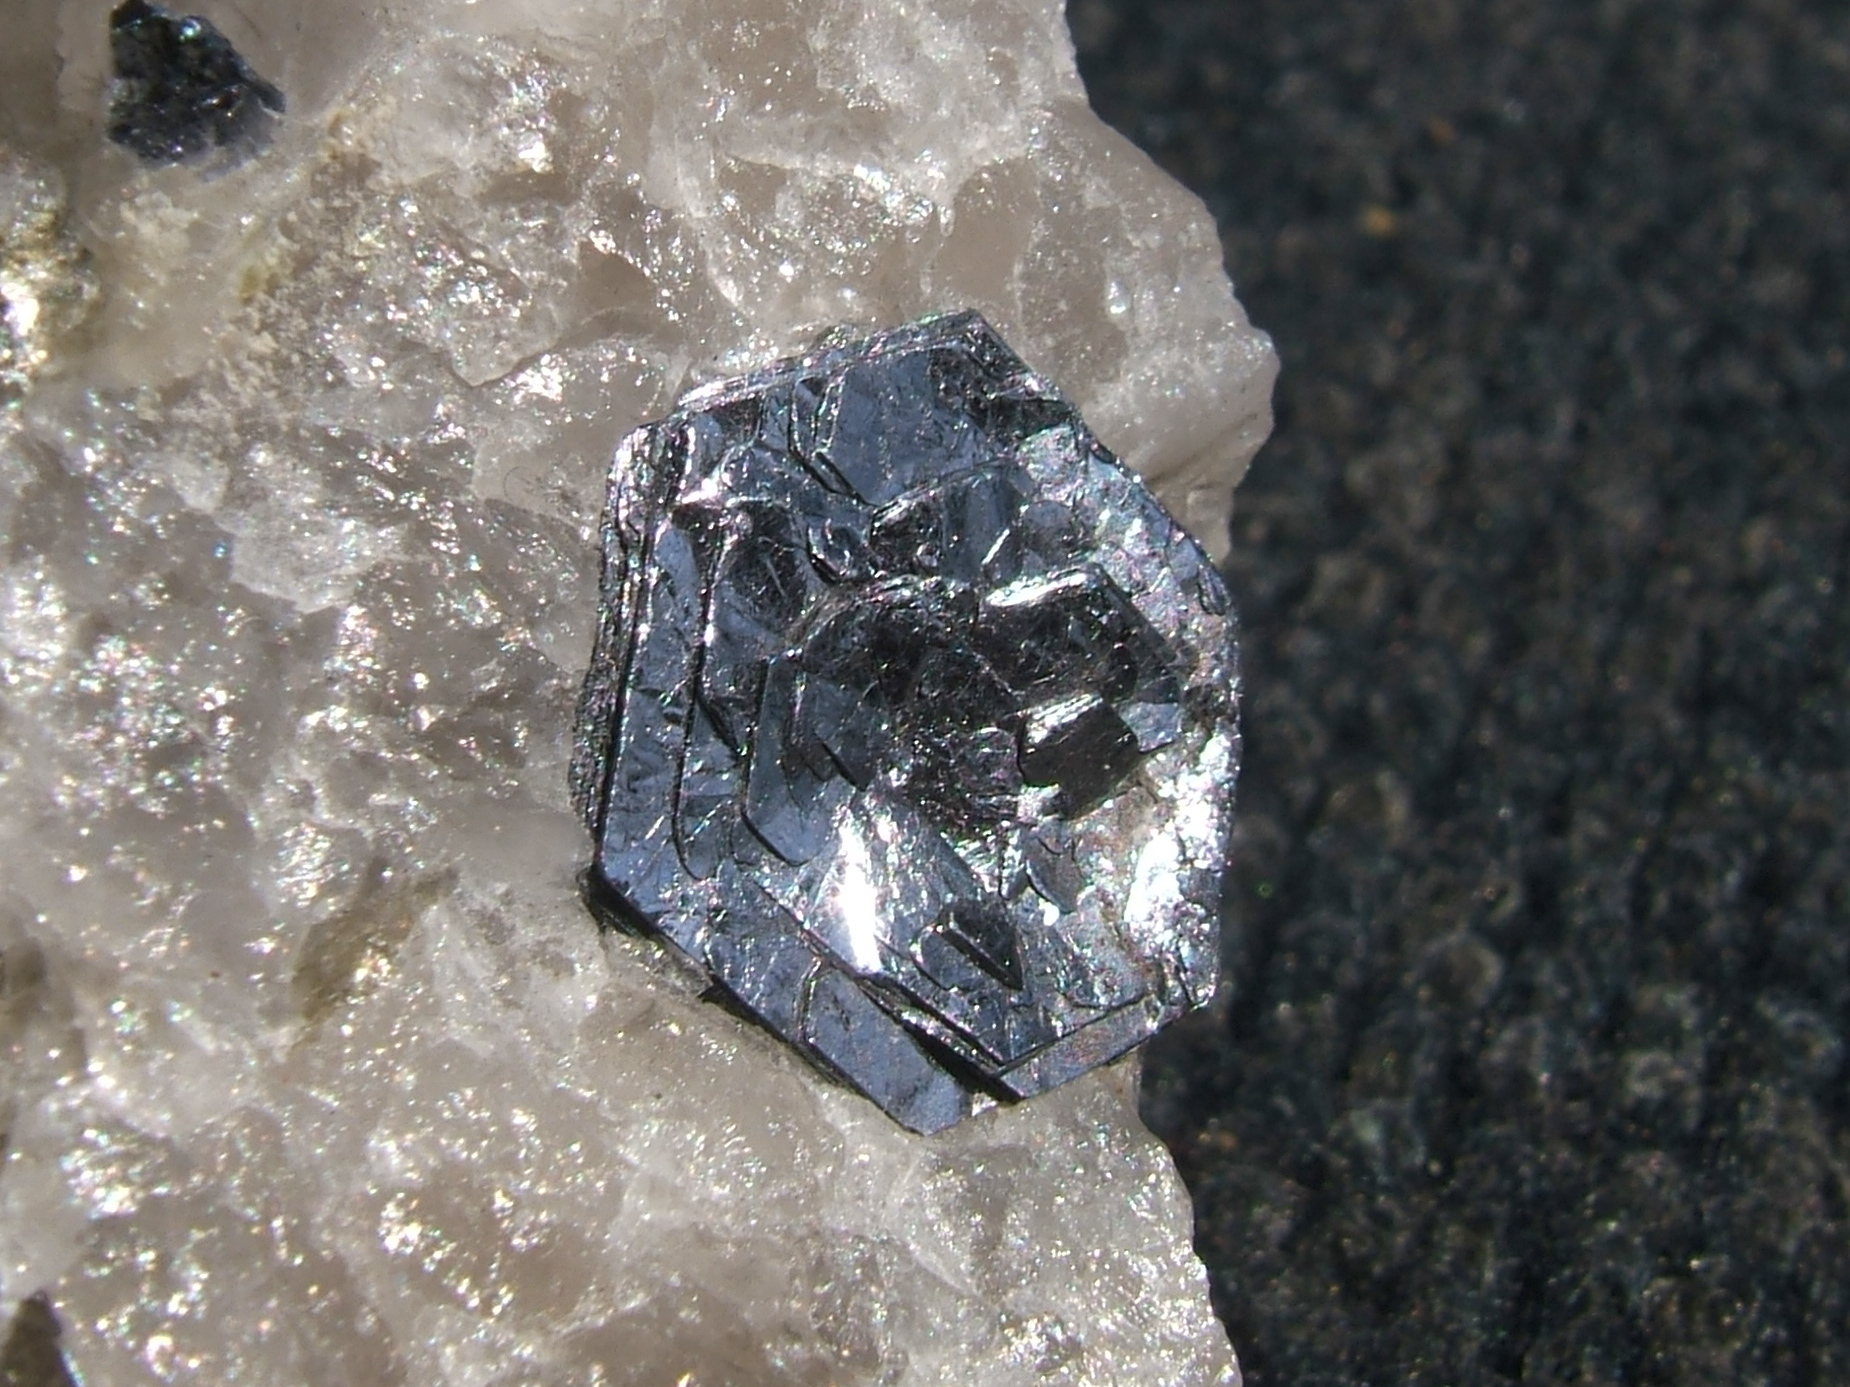
\includegraphics[width=1.0\linewidth]{imagens/molybdenite.jpeg}
      \caption{}
      \label{fig:mos2a}
    \end{subfigure}
    \begin{subfigure}{0.49\textwidth}
      \centering
      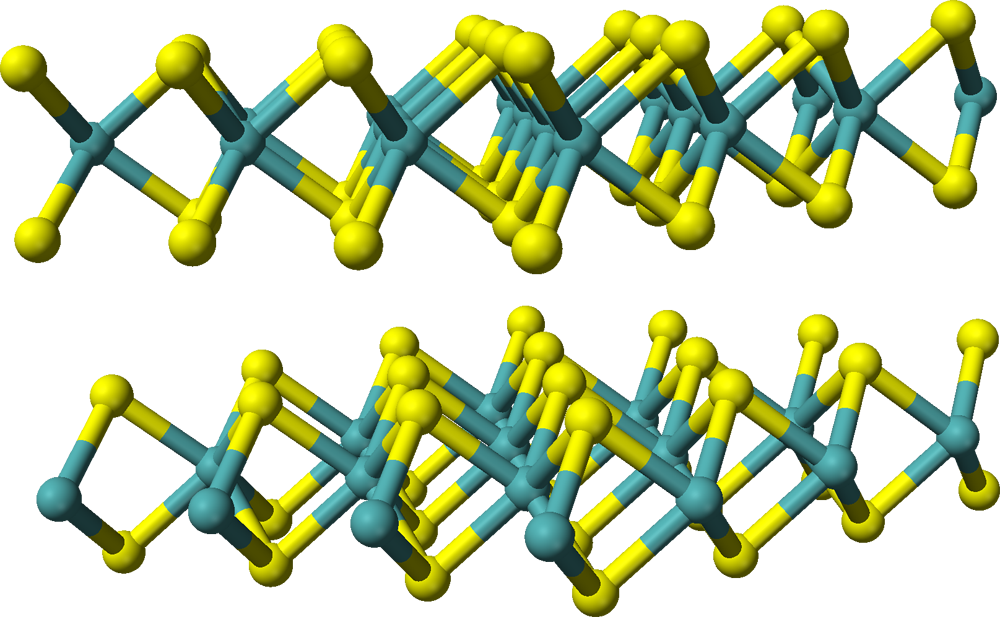
\includegraphics[width=1.0\linewidth]{imagens/molybdenite_crystal.png}
      \caption{}
      \label{fig:mos2b}
    \end{subfigure}
    \caption{
      \subref{fig:mos2a} Molibdenita incrustada em uma massa de quartzo.
      \subref{fig:mos2b} Representação da estrutura cristalina da molibdenita. Molibdênio em azul, enxofre em amarelo.
    }
    \label{fig:mos2}
  \end{figure}
\end{frame}

\begin{frame}{Dicalcogenetos de Metais de Transição}
  \begin{itemize}
    \item Para aplicações, é de fundamental importância o conhecimento sobre a
          estrutura eletrônica do material
    \item Em especial, é importante o conhecimento do \textit{bandgap} do cristal
    \item Este valor é a diferença entre o menor nível da banda de condução e o
          maior nível da banda de valência
    \item Essa é a energia de um éxciton produzido pela excitação de um elétron de valência
  \end{itemize}
  \begin{block}{}
    \centering
    Um éxciton é um par elétron-buraco formado pela transição de um elétron de
    valência para uma camada de condução
  \end{block}
\end{frame}

\begin{frame}{Dicalcogenetos de Metais de Transição}
  \begin{itemize}
    \item Usualmente, as bandas são calculadas ao longo da primeira zona de
          Brillouin do cristal
    \item Essa região é a correspondente da  célula primitiva de Wigner-Seitz na rede
          recíproca
    \item A rede recíproca pode ser vista como a transformada de Fourier da rede
          primitiva
  \end{itemize}
\end{frame}

\begin{frame}{Dicalcogenetos de Metais de Transição}
  \begin{figure}
    \begin{columns}
      \begin{column}{0.35\textwidth}
        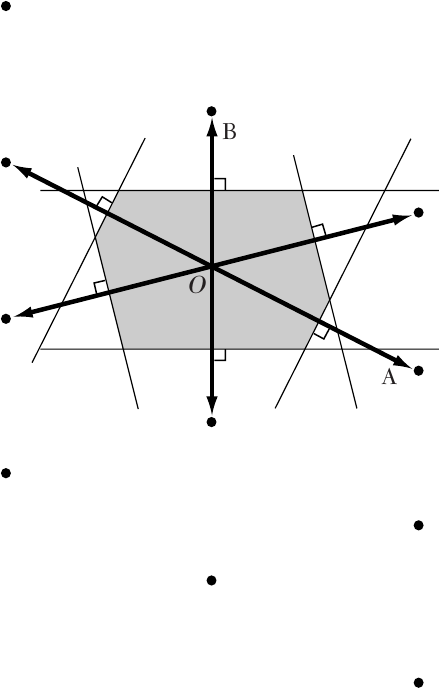
\includegraphics[width=\textwidth]{imagens/brillouin.png}
      \end{column}
      \begin{column}{0.65\textwidth}
        \caption{
          A primeira zona de Brillouin é obtida da seguinte forma: primeiro,
          traçamos segmentos de reta de $O$ até os pontos vizinhos na rede
          recíproca. Em seguida traçamos os planos mediadores de cada um desses
          segmentos. O volume delimitado corresponde à região desejada.
        }
      \end{column}
    \end{columns}
  \end{figure}
\end{frame}

\begin{frame}{Dicalcogenetos de Metais de Transição}
  \newcommand\xsla{-1.2}
\newcommand\ysla{0.505}
\newcommand\hexheight{3em}
\newcommand\hexside{2em}

\newcommand\hex[3][]{
  \begin{scope}[
      #1,
      xscale=-1,
      yshift=#3,
      yslant=\ysla,
      xslant=\xsla,
      every node/.style={anchor=west,regular polygon,regular polygon sides=6,draw,inner sep=\hexside},
      transform shape
    ]
    \node (hex_#2) {};
  \end{scope}
}

\newcommand\hexhidden[3][]{
  \begin{scope}[
      #1,
      xscale=-1,
      yshift=#3,
      yslant=\ysla,
      xslant=\xsla,
      every node/.style={anchor=west,regular polygon,regular polygon sides=6,inner sep=\hexside,draw,dotted},
      transform shape
    ]
    \node (hex_#2) {};
  \end{scope}
}

\begin{figure}[b]
  \centering
  \begin{tikzpicture}
    \hex{top}{\hexheight}
    \hexhidden{middle}{0}
    \hex{bottom}{-\hexheight}

    \foreach \corn in {1,...,6}
    \draw (hex_top.corner \corn) -- (hex_bottom.corner \corn);

    % Caminho no qual as bandas são calculadas
    \draw[thick,myarrow=0.5] (hex_middle.center) -- (hex_middle.corner 4);
    \draw[thick,myarrow=0.5] (hex_middle.corner 4) -- (hex_middle.side 3);

    % Pontos de simetria
    \draw[fill=black] (hex_middle.center) circle (2pt) node[right]{$\Gamma$};
    \draw[fill=black] (hex_middle.corner 4) circle (2pt) node[below left]{$K$};
    \draw[fill=black] (hex_middle.side 3) circle (2pt) node[below right]{$M$};
    \draw[fill=black] (hex_middle.corner 3) circle (2pt) node[above right]{$K'$};
    \draw[fill=black] (hex_top.center) circle (2pt) node[above right]{$A$};
  \end{tikzpicture}
  \caption{
    Zona de Brillouin para monocamadas de TMDCs e principais pontos de simetria.
    Geralmente as bandas de valência e de condução são calculadas ao longo desses
    pontos, como no caminho exemplificado.
  }
  \label{fig:brillouin}
\end{figure}
\end{frame}

\begin{frame}{Dicalcogenetos de Metais de Transição}
  \begin{figure}
    \centering
    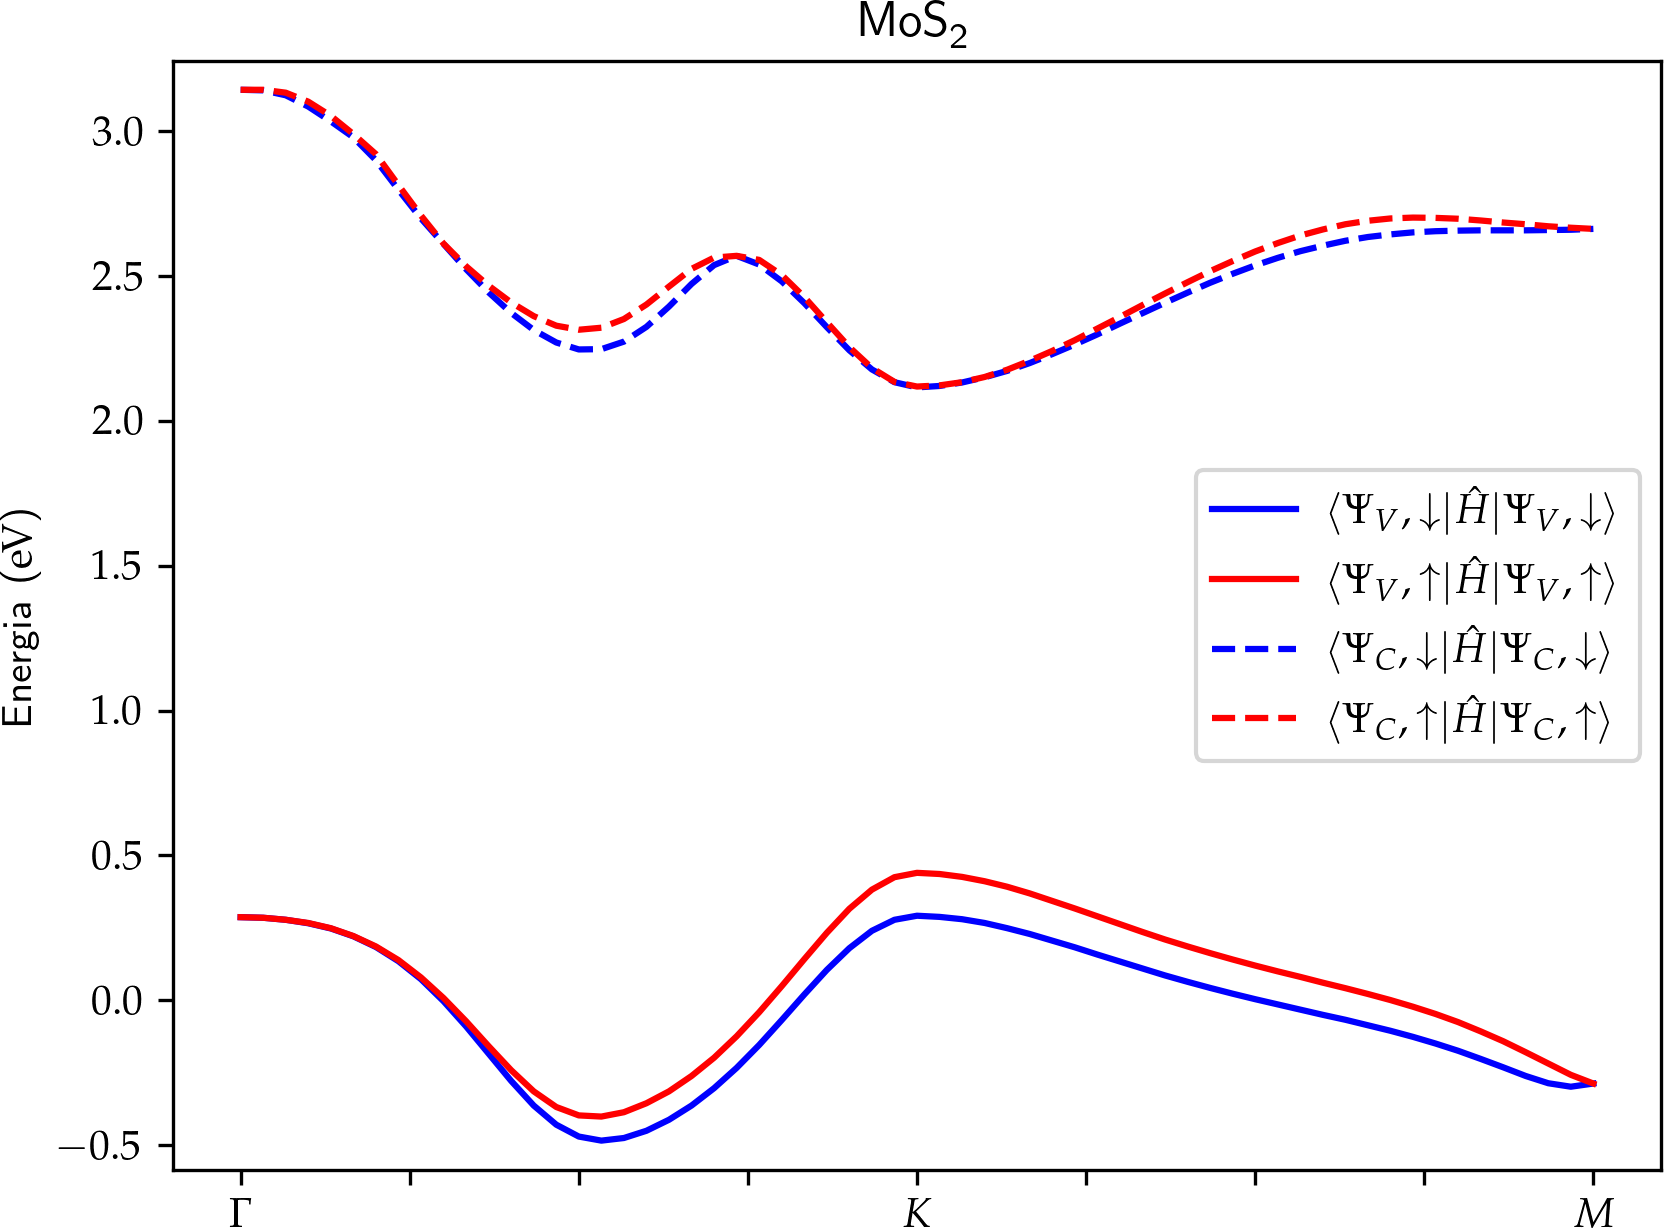
\includegraphics[height=0.68\textheight]{imagens/mos2_bands.png}
    \caption{
      Energias das bandas de condução e de valência ao longo do caminho
      $\Gamma$-$K$-$M$ para o dissulfeto de molibdênio, calculadas via DFT.
    }
    \label{fig:mos2_bands}
  \end{figure}
\end{frame}

\begin{frame}{O Modelo $k \cdot p$}
  \begin{itemize}
    \item Aproxima as bandas em torno dos vales $K$ e $K'$
    \item É um modelo analítico, o que facilita o desenvolvimento de uma
          intuição física acerca do material, possibilitando a observação do
          comportamento das bandas de energia com a variação dos parâmetros que
          as descrevem
    \item Computacionalmente barato
    \item Possibilidade de inclusão de um campo magnético normal à monocamada do
          material à descrição do sistema, o que tornaria impraticável o uso do DFT
  \end{itemize}
\end{frame}

\begin{frame}{O Modelo $k \cdot p$}
  \begin{itemize}
    \item As bandas são dadas na base
          $$ \left\{ \ket{\Psi_C,\uparrow} ; \ket{\Psi_C,\downarrow} ; \ket{\Psi_V,\uparrow} ; \ket{\Psi_V,\downarrow} \right\} $$
          pelos autovalores de
          $$ \hat{H}_{kp}(\bvec{k}) = \hat{H}_0 + \sum_{i=1}^3 \hat{H}_{kp}^{(i)}(\bvec{k}) $$
    \item O vetor $\bvec{k}$ é uma posição na zona de Brillouin
  \end{itemize}
\end{frame}

\begin{frame}
  \tiny
  \begin{align*}
    \begin{split}
      & \hat{H}_0 =
      \left(
      \begin{matrix}
          E_F + \Delta - \tau \lambda_c & 0                    & 0                             & 0                    \\
          0                             & E_F + \tau \lambda_v & 0                             & 0                    \\
          0                             & 0                    & E_F + \Delta + \tau \lambda_c & 0                    \\
          0                             & 0                    & 0                             & E_F - \tau \lambda_v \\
        \end{matrix}
      \right) \\
      & \hat{H}_{kp}^{(1)}(\bvec{k}) =
      \left(
      \begin{matrix}
          0                                     & \gamma_0 f_1(\bvec{k},\tau) & 0                                     & 0                           \\
          \gamma_0 f_1^{\dagger}(\bvec{k},\tau) & 0                           & 0                                     & 0                           \\
          0                                     & 0                           & 0                                     & \gamma_0 f_1(\bvec{k},\tau) \\
          0                                     & 0                           & \gamma_0 f_1^{\dagger}(\bvec{k},\tau) & 0                           \\
        \end{matrix}
      \right) \\
      & \hat{H}_{kp}^{(2)}(\bvec{k}) =
      \left(
      \begin{matrix}
          \gamma_1 f_2(\bvec{k})                & \gamma_3 f_3(\bvec{k},\tau) & 0                                     & 0                           \\
          \gamma_3 f_3^{\dagger}(\bvec{k},\tau) & \gamma_2 f_2(\bvec{k})      & 0                                     & 0                           \\
          0                                     & 0                           & \gamma_1 f_2(\bvec{k})                & \gamma_3 f_3(\bvec{k},\tau) \\
          0                                     & 0                           & \gamma_3 f_3^{\dagger}(\bvec{k},\tau) & \gamma_2 f_2(\bvec{k})      \\
        \end{matrix}
      \right) \\
      & \hat{H}_{kp}^{(3)}(\bvec{k}) =
      \left(
      \begin{matrix}
          \gamma_4 f_4(\bvec{k})                & \gamma_6 f_5(\bvec{k},\tau) & 0                                     & 0                           \\
          \gamma_6 f_5^{\dagger}(\bvec{k},\tau) & \gamma_5 f_4(\bvec{k})      & 0                                     & 0                           \\
          0                                     & 0                           & \gamma_4 f_4(\bvec{k})                & \gamma_6 f_5(\bvec{k},\tau) \\
          0                                     & 0                           & \gamma_6 f_5^{\dagger}(\bvec{k},\tau) & \gamma_5 f_4(\bvec{k})      \\
        \end{matrix}
      \right)
    \end{split}
  \end{align*}
  \begin{align*}
    \begin{split}
      & f_1(\bvec{k},\tau) = a(\tau k_x - i k_y)                    \\
      & f_2(\bvec{k}) = a^2(k_x^2 + k_y^2)                          \\
      & f_3(\bvec{k},\tau) = a^2(\tau k_x + i k_y)^2                \\
      & f_4(\bvec{k},\tau) = a^3 \tau k_x (k_x^2 - 3 k_y^2)         \\
      & f_5(\bvec{k},\tau) = a^3 (k_x^2 + k_y^2) (\tau k_x - i k_y)
    \end{split}
  \end{align*}
  \normalsize
\end{frame}

\begin{frame}{O Modelo $k \cdot p$}
  \begin{block}{Como usar esse modelo?}
    \begin{itemize}
      \item Suponha que tenhamos uma sequencia de valores das bandas ao longo de
            $\Gamma$-$K$-$M$, tendo pontos na vizinhança de $K$
      \item Esses valores podem ser obtidos usando DFT, por exemplo
      \item Vamos denotar por $ E_{ik}^{(dft)} $ o $i$-ésimo maior valor de
            energia no $k$-ésimo ponto
      \item Podemos usar o modelo para inferir os valores dos parâmetros que descrevem o cristal
    \end{itemize}
  \end{block}
\end{frame}

\begin{frame}{O Modelo $k \cdot p$}
  \begin{block}{Como usar esse modelo?}
    \begin{itemize}
      \item Os parâmetros que melhor ajustam o modelo podem ser encontrados
            usando o método dos mínimos quadrados
      \item Procuramos os parâmetros que minimizem
            $$
              f(E_F, \Delta, \lambda_c, \lambda_v, \gamma_i) =
              \frac{1}{4 N} \sum_{k=1}^N \sum_{i=1}^4 \left( E_{ik}^{(dft)} - E_{ik}^{(kp)} \right)^2
            $$
            sendo $E_{ik}^{(kp)}$ o $i$-ésimo maior autovalor de $\hat{H}_{kp}$
    \end{itemize}
  \end{block}
\end{frame}

\begin{frame}{O Modelo $k \cdot p$}
  \begin{block}{Como usar esse modelo?}
    \begin{itemize}
      \item Para obter o valor de $f$ então é preciso obter os autovalores da
            Hamiltoniana e em seguida ordená-los
      \item Isso sugere o uso de métodos de busca estocásticos
      \item Usaremos o Algoritmo Genético desenvolvido para buscar um mínimo
            para $f$
    \end{itemize}
  \end{block}
\end{frame}

\section{Resultados}

\begin{frame}{Ajuste das Bandas dos Cristais \ch{CrS2} e \ch{CrSe2}}
  \begin{block}{Parâmetros Usados no Algorítmo para o Ajuste}
    \begin{itemize}
      \item 16 processos concorrentes
      \item 1000 indivíduos por processo, evoluídos por 200 gerações
      \item $p_2 = p_3 = 5\%$, $h = 2$, $e_1 = 5\%$ e $e_2 = e_3 = 10\%$
    \end{itemize}
    \begin{table}
      \centering
      \begin{tabular}{lrr}
        \toprule
                    & Mínimo     & Máximo    \\
        \midrule
        $E_F$       & \num{-1.0} & \num{1.0} \\
        $\Delta$    & \num{0.5}  & \num{1.2} \\
        $\lambda_c$ & \num{0.0}  & \num{1.0} \\
        $\lambda_v$ & \num{0.0}  & \num{1.0} \\
        $\gamma_i$  & \num{-1.0} & \num{1.0} \\
        \bottomrule
      \end{tabular}
    \end{table}
  \end{block}
\end{frame}

\begin{frame}{Ajuste das Bandas dos Cristais \ch{CrS2} e \ch{CrSe2}}
  \begin{table}
    \centering
    \begin{tabular}{lcc}
      \toprule
                                         & \ch{CrS2}         & \ch{CrSe2}        \\
      \midrule
      $ a \; (\si{\angstrom}) $          & \num{3.022302679} & \num{3.167287237} \\
      $ \Delta \; (\si{\electronvolt}) $ & \num{0.942}       & \num{0.763}       \\
      \bottomrule
    \end{tabular}
    \caption{
      Valores para os parâmetros de rede considerados nos processos de otimização
      e valores esperados para o \textit{bandgap}, para cada um dos materiais
      considerados.
    }
    \label{tab:lattice_delta}
  \end{table}
\end{frame}

\begin{frame}{Ajuste das Bandas dos Cristais \ch{CrS2} e \ch{CrSe2}}
  \begin{table}
    \resizebox*{0.58\textwidth}{!}{\begin{tabular}{lrrrr}
\toprule
{} & \multicolumn{2}{c}{Algorítmo Genético} & \multicolumn{2}{c}{\textit{Dual Annealing}} \\
{} &           1ª Ordem &  3ª Ordem &                1ª Ordem &  3ª Ordem \\
\midrule
$f$         &           0,003858 &  0,000335 &                0,003860 &  0,000165 \\
$E_F$       &          -0,052734 &  0,023191 &               -0,052109 &  0,010791 \\
$\Delta$    &           1,077500 &  0,954347 &                1,076284 &  0,976370 \\
$\lambda_c$ &          -0,002289 &  0,006503 &                0,000000 &  0,000000 \\
$\lambda_v$ &           0,031810 &  0,030079 &                0,032250 &  0,033154 \\
$\gamma_0$  &           0,475147 &  0,508048 &               -0,475765 &  0,662441 \\
$\gamma_1$  &                    &  0,227823 &                         &  0,038586 \\
$\gamma_2$  &                    & -0,216329 &                         & -0,050962 \\
$\gamma_3$  &                    &  0,185349 &                         &  0,196977 \\
$\gamma_4$  &                    & -0,063952 &                         & -0,128763 \\
$\gamma_5$  &                    &  0,037538 &                         &  0,116953 \\
$\gamma_6$  &                    & -0,196858 &                         & -0,147924 \\
\bottomrule
\end{tabular}
}
    \caption{
      Parâmetros da Hamiltoniana $ \hat{H}_{kp} $ ajustados para \ch{CrS2}
      usando as expansões de 1ª e 3ª ordem, bem como os valores para a função
      objetivo $f$ correspondente.
    }
  \end{table}
\end{frame}

\begin{frame}{Ajuste das Bandas dos Cristais \ch{CrS2} e \ch{CrSe2}}
  \begin{table}
    \resizebox*{0.58\textwidth}{!}{\begin{tabular}{lrrrr}
\toprule
{} & \multicolumn{2}{c}{Algorítmo Genético} & \multicolumn{2}{c}{\textit{Dual Annealing}} \\
{} &           1ª Ordem &  3ª Ordem &                1ª Ordem &  3ª Ordem \\
\midrule
$f$         &           0,002695 &  0,000261 &                0,002695 &  0,000129 \\
$E_F$       &           0,657808 &  0,722708 &                0,657704 &  0,715254 \\
$\Delta$    &           0,897031 &  0,792868 &                0,896809 &  0,814547 \\
$\lambda_c$ &           0,006592 &  0,007456 &                0,006680 &  0,007329 \\
$\lambda_v$ &           0,045311 &  0,047549 &                0,045330 &  0,042298 \\
$\gamma_0$  &          -0,381442 & -0,649511 &                0,381519 &  0,456269 \\
$\gamma_1$  &                    & -0,090387 &                         &  0,137704 \\
$\gamma_2$  &                    &  0,090028 &                         & -0,154747 \\
$\gamma_3$  &                    & -0,075382 &                         &  0,124848 \\
$\gamma_4$  &                    & -0,059988 &                         & -0,030592 \\
$\gamma_5$  &                    &  0,037979 &                         &  0,016737 \\
$\gamma_6$  &                    &  0,110312 &                         & -0,169387 \\
\bottomrule
\end{tabular}
}
    \caption{
      Parâmetros da Hamiltoniana $ \hat{H}_{kp} $ ajustados para \ch{CrSe2}
      usando as expansões de 1ª e 3ª ordem, bem como os valores para a função
      objetivo $f$ correspondente.
    }
  \end{table}
\end{frame}

\begin{frame}{Ajuste das Bandas dos Cristais \ch{CrS2} e \ch{CrSe2}}
  \begin{figure}
    \centering
    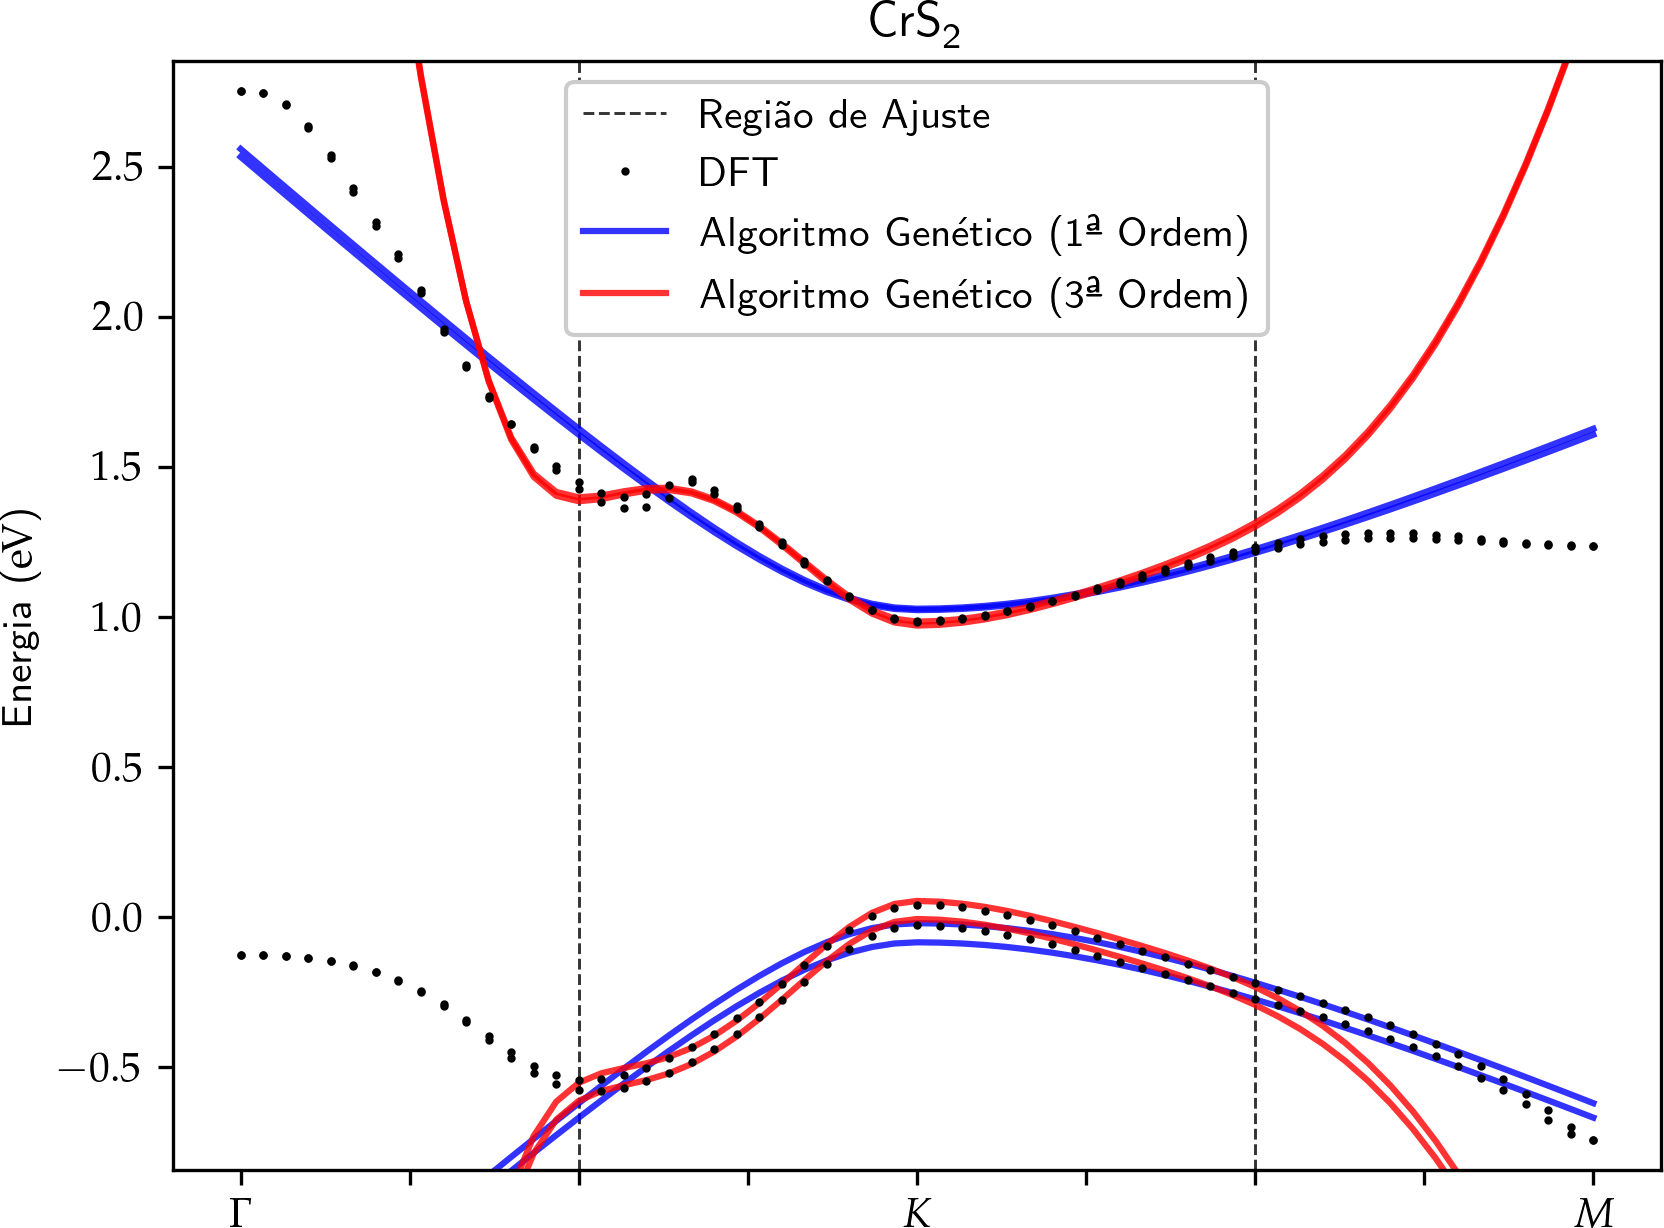
\includegraphics[width=0.68\textwidth]{imagens/crs2_genetic_algorithm_order_13.png}
    \caption{
      Gráficos das bandas de energia ajustadas para \ch{CrS2} via Algoritmo Genético
      usando as expansões de 1ª e 3ª ordem de $ \hat{H}_{kp} $.
    }
  \end{figure}
\end{frame}

\begin{frame}{Ajuste das Bandas dos Cristais \ch{CrS2} e \ch{CrSe2}}
  \begin{figure}
    \centering
    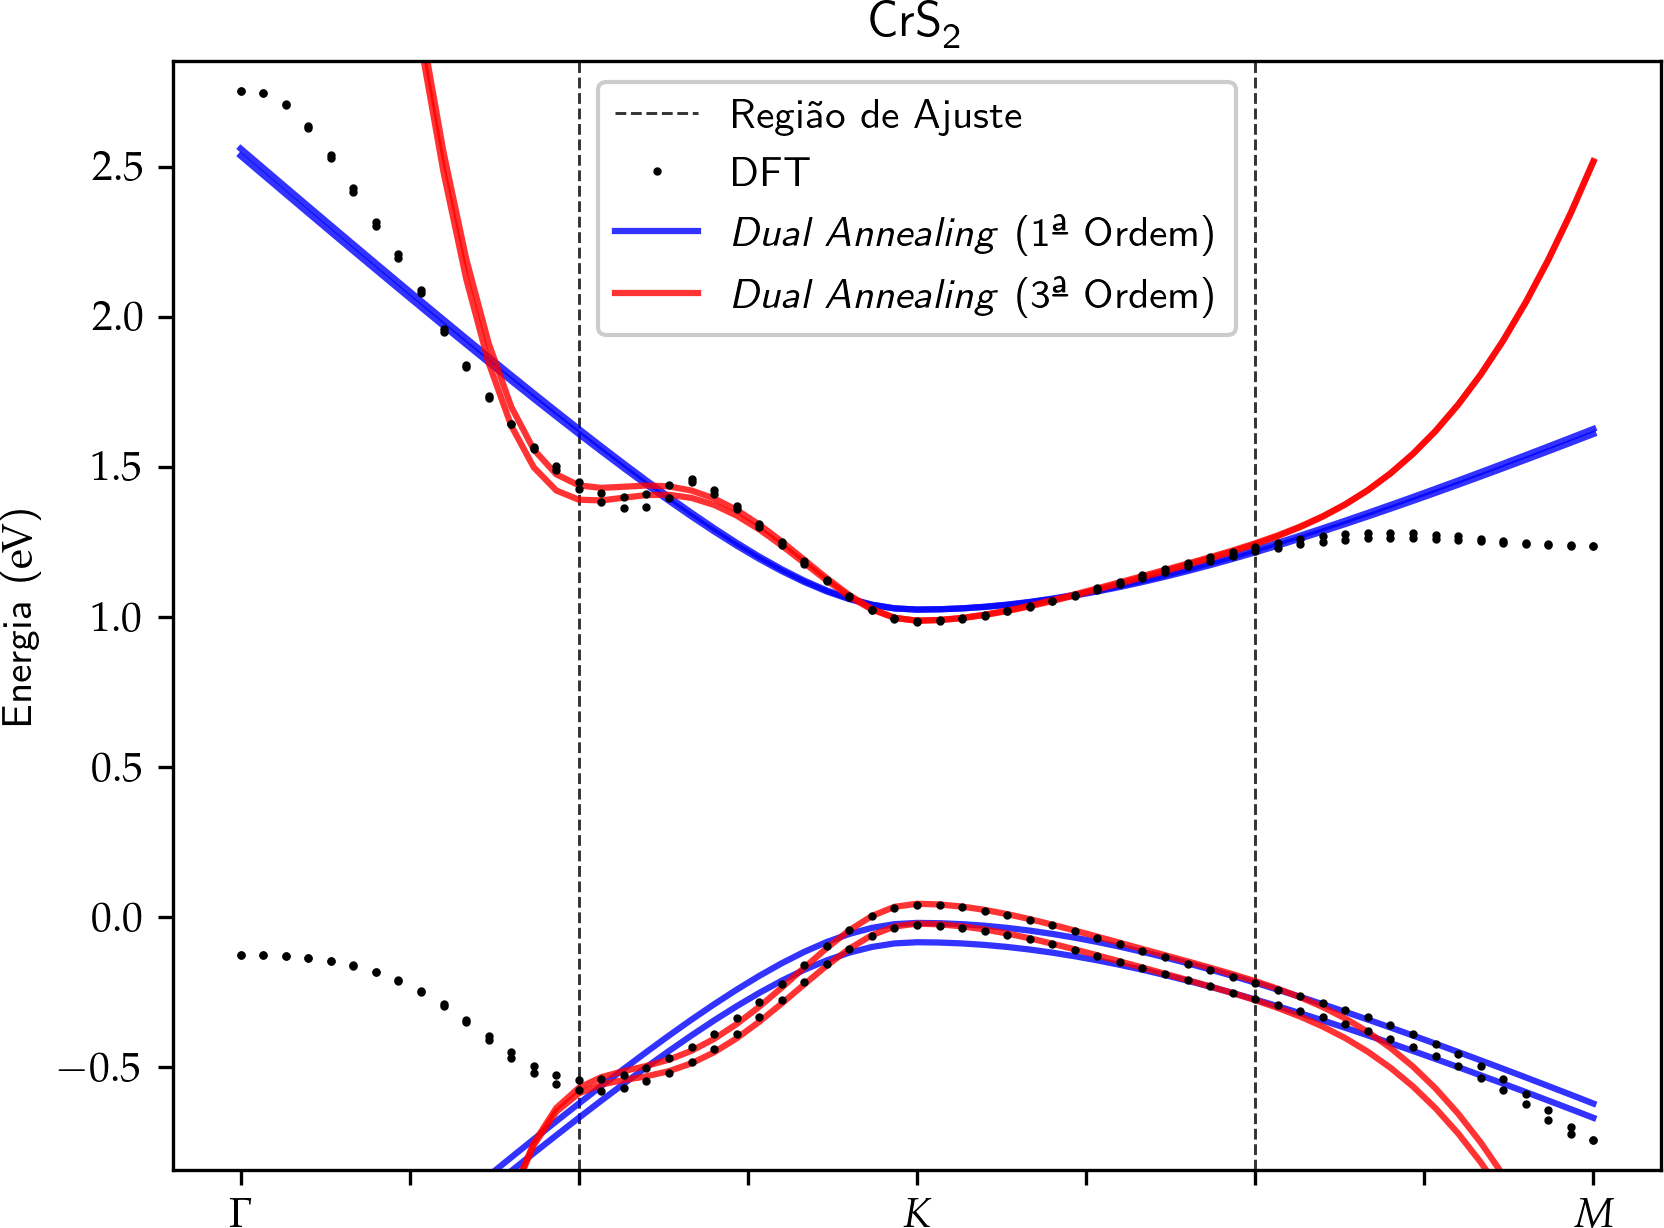
\includegraphics[width=0.68\textwidth]{imagens/crs2_dual_annealing_order_13.png}
    \caption{
      Gráficos das bandas de energia ajustadas para \ch{CrS2} via \textit{Dual Annealing}
      usando as expansões de 1ª e 3ª ordem de $ \hat{H}_{kp} $.
    }
  \end{figure}
\end{frame}

\begin{frame}{Ajuste das Bandas dos Cristais \ch{CrS2} e \ch{CrSe2}}
  \begin{figure}
    \centering
    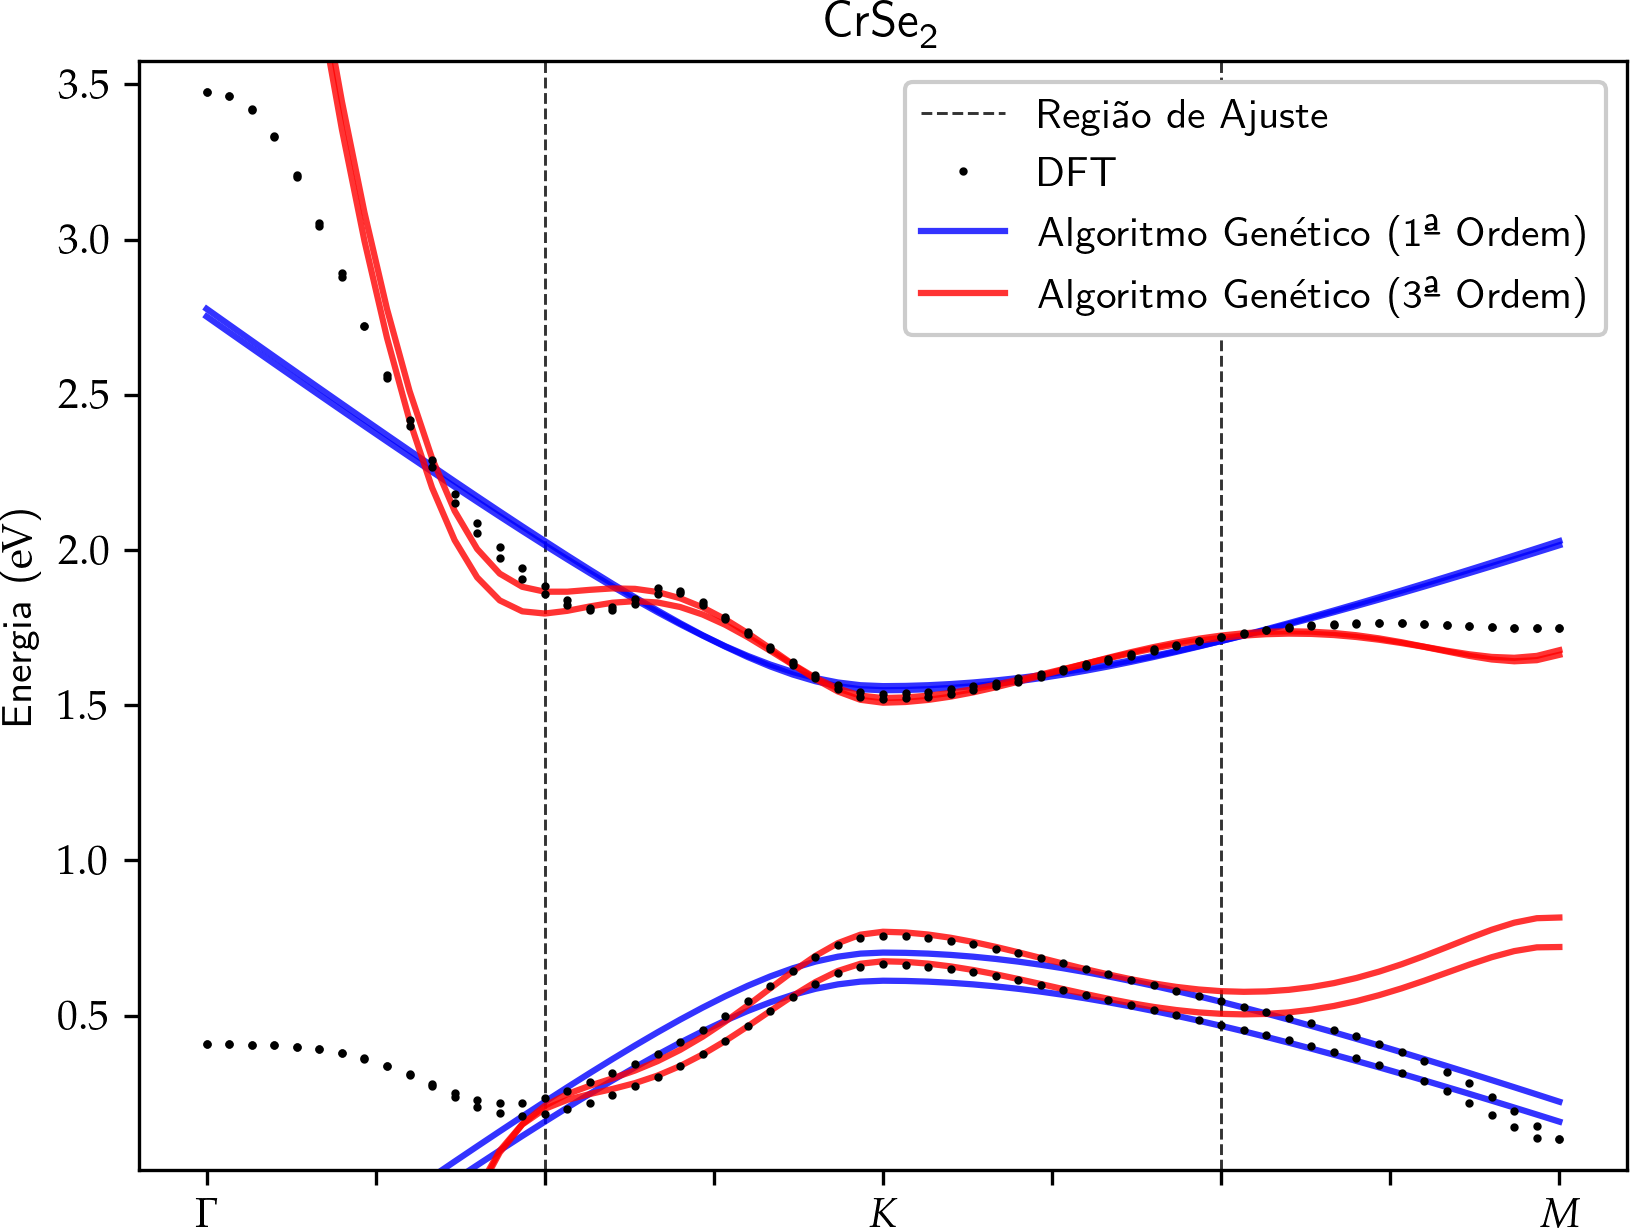
\includegraphics[width=0.68\textwidth]{imagens/crse2_genetic_algorithm_order_13.png}
    \caption{
      Gráficos das bandas de energia ajustadas para \ch{CrSe2} via Algoritmo Genético
      usando as expansões de 1ª e 3ª ordem de $ \hat{H}_{kp} $.
    }
  \end{figure}
\end{frame}

\begin{frame}{Ajuste das Bandas dos Cristais \ch{CrS2} e \ch{CrSe2}}
  \begin{figure}
    \centering
    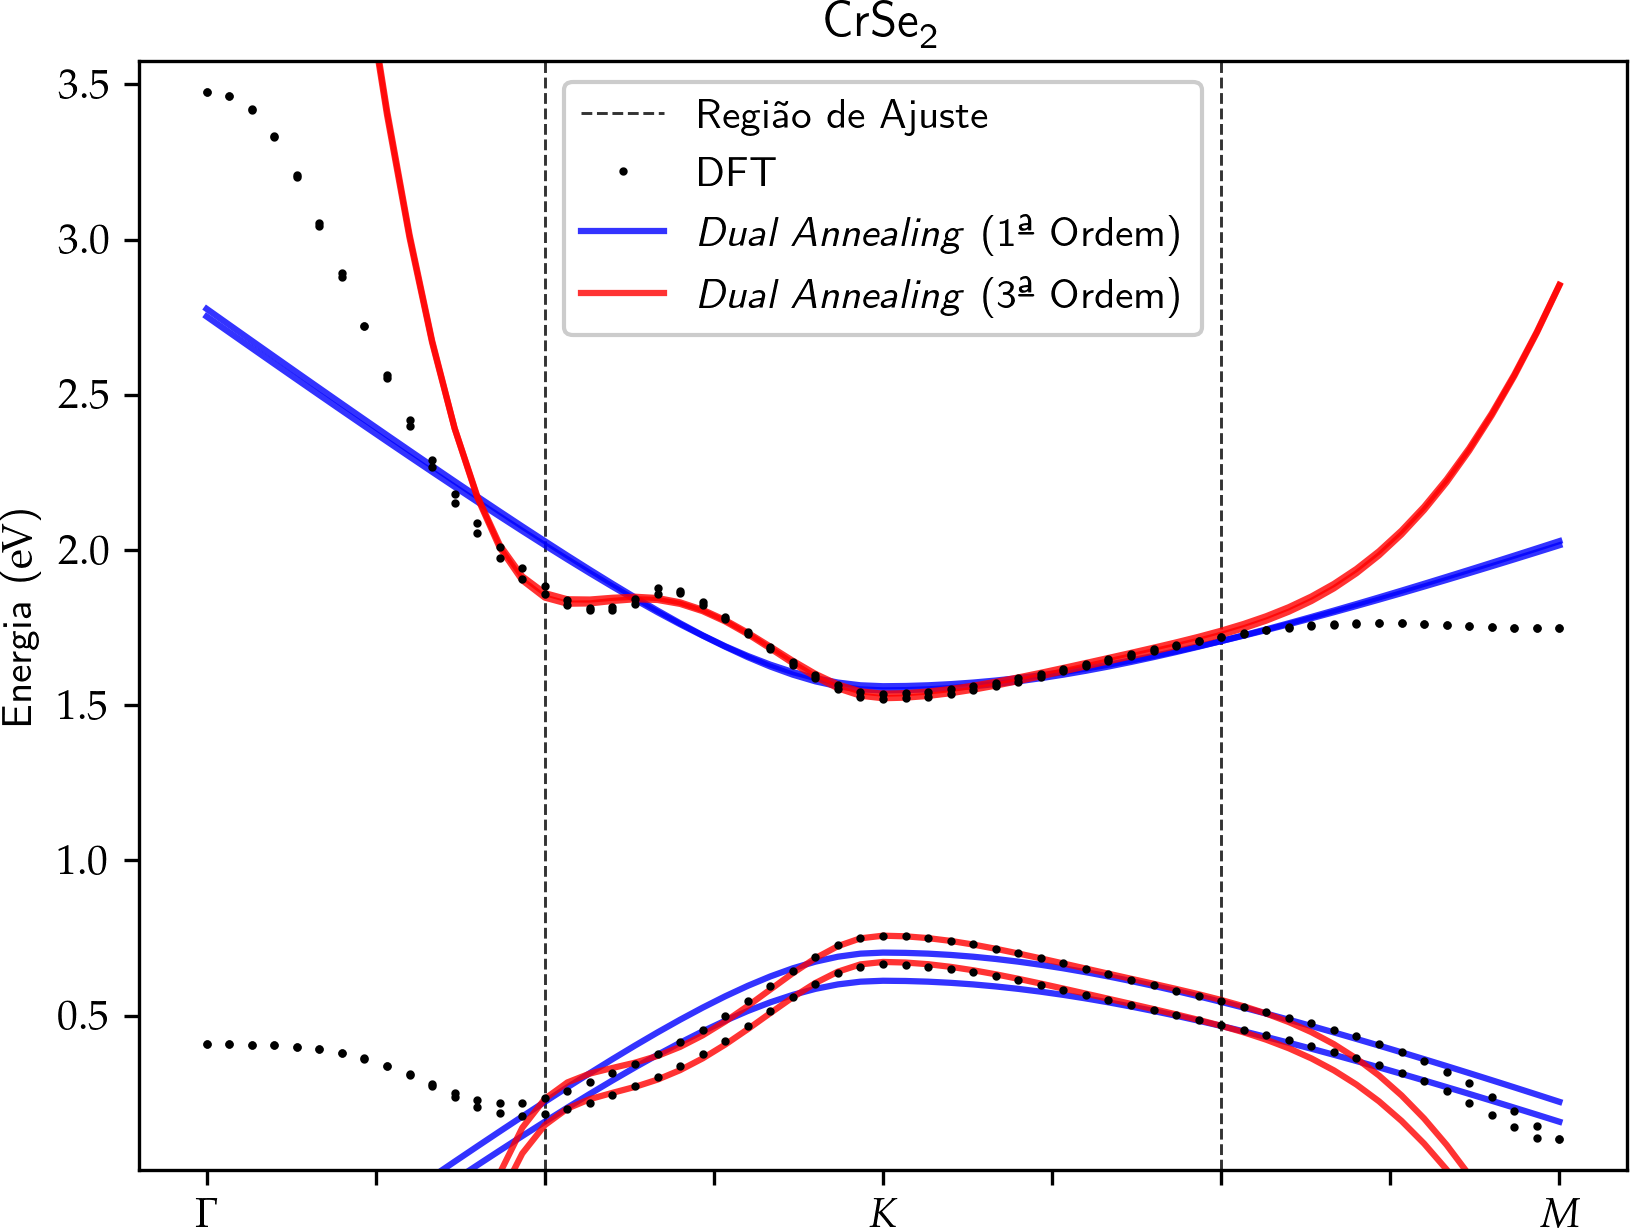
\includegraphics[width=0.68\textwidth]{imagens/crse2_dual_annealing_order_13.png}
    \caption{
      Gráficos das bandas de energia ajustadas para \ch{CrSe2} via \textit{Dual Annealing}
      usando as expansões de 1ª e 3ª ordem de $ \hat{H}_{kp} $.
    }
  \end{figure}
\end{frame}

\begin{frame}{Níveis de Landau}
  \begin{itemize}
    \item Podemos estudar o comportamento do \textit{bandgap} dos materiais em
          questão sob o efeito de um campo magnético $B$ normal à monocamada
    \item Adicionando o termo de iteração à expansão de 1ª ordem e calculando os
          seus autovalores, obtemos
          \begin{align*}
             & E_\pm (B, n, s_z) = \frac{\lambda_v \tau s_z}{2} \pm
            \sqrt{
              \frac{(\Delta - \lambda_v \tau s_z)^2}{4} +
              \frac{2 \gamma_0^2 a^2 e B n}{\hbar}
            }
            \\
             & E_{(n = 0)} =
            \begin{cases}
              - \nicefrac{\Delta}{2} + \lambda_v s_z \;, & \text{se } \tau = 1 \quad \text{(valência)}  \\
              \nicefrac{\Delta}{2}                   \;, & \text{se } \tau = -1 \quad \text{(condução)} \\
            \end{cases}
            \\
          \end{align*}
  \end{itemize}
\end{frame}

\begin{frame}{Níveis de Landau}
  \begin{figure}
    \centering
    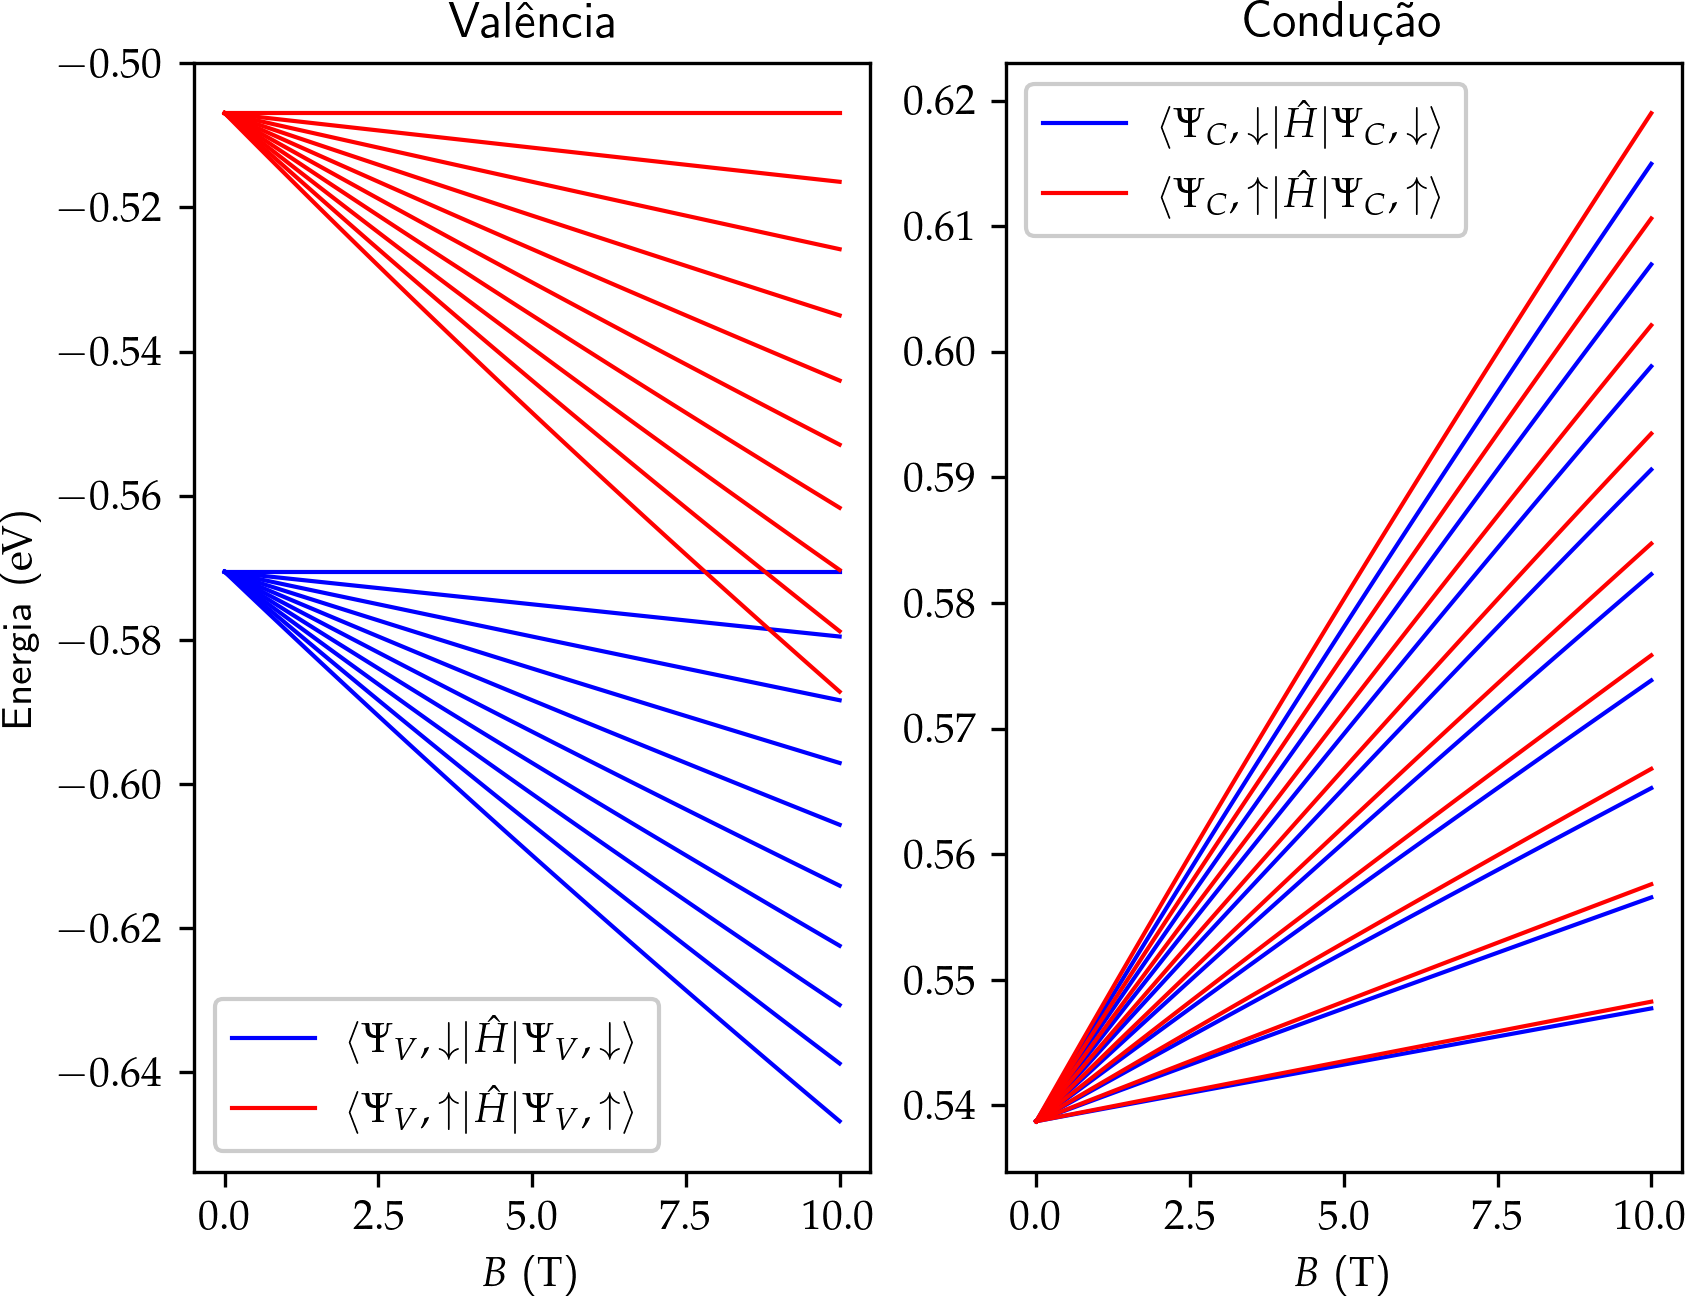
\includegraphics[width=0.68\textwidth]{imagens/crs2_k_valley_landau_levels.png}
    \caption{Níveis de Landau no vale $K$ para \ch{CrS2} em termos de $B$.}
  \end{figure}
\end{frame}

\begin{frame}{Níveis de Landau}
  \begin{figure}
    \centering
    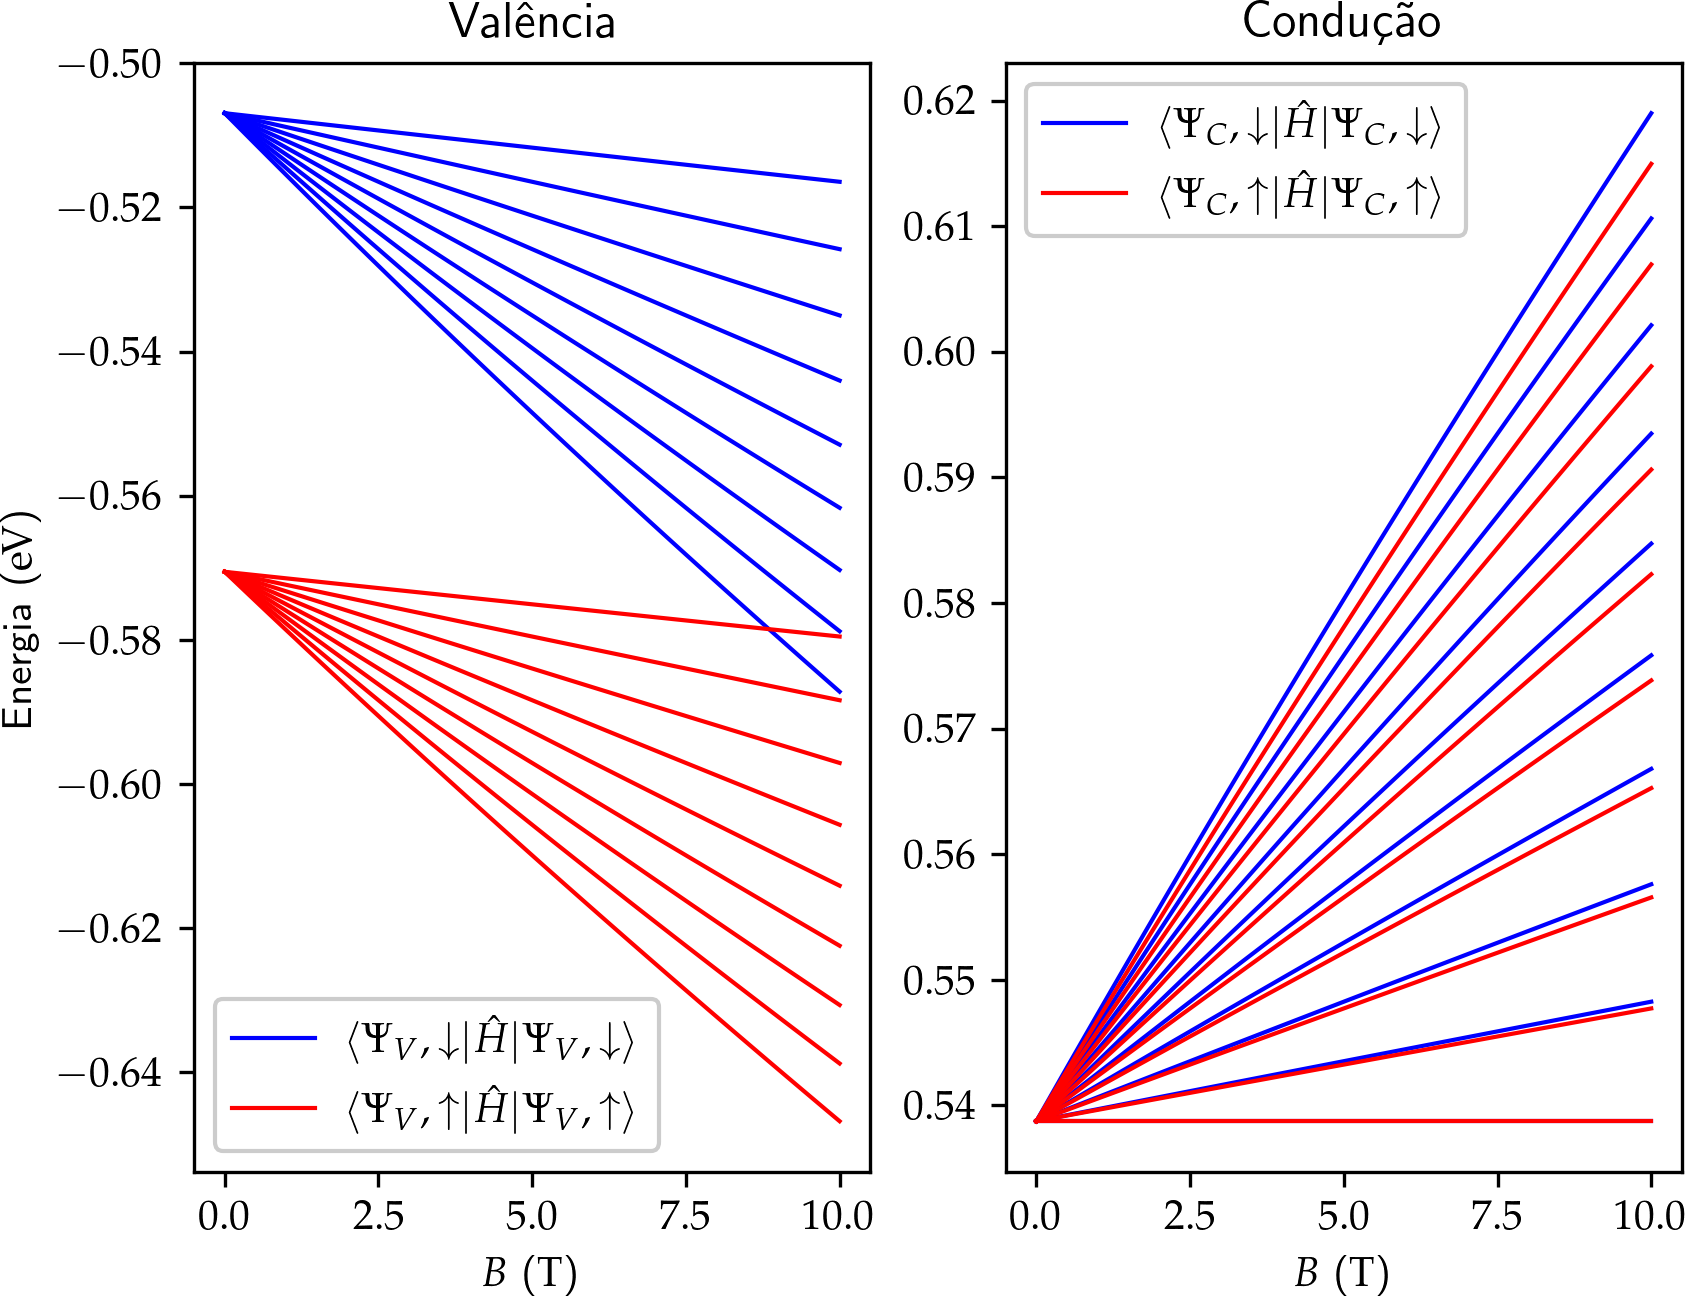
\includegraphics[width=0.68\textwidth]{imagens/crs2_k_prime_valley_landau_levels.png}
    \caption{Níveis de Landau no vale $K'$ para \ch{CrS2} em termos de $B$.}
  \end{figure}
\end{frame}

\begin{frame}{Níveis de Landau}
  \begin{figure}
    \centering
    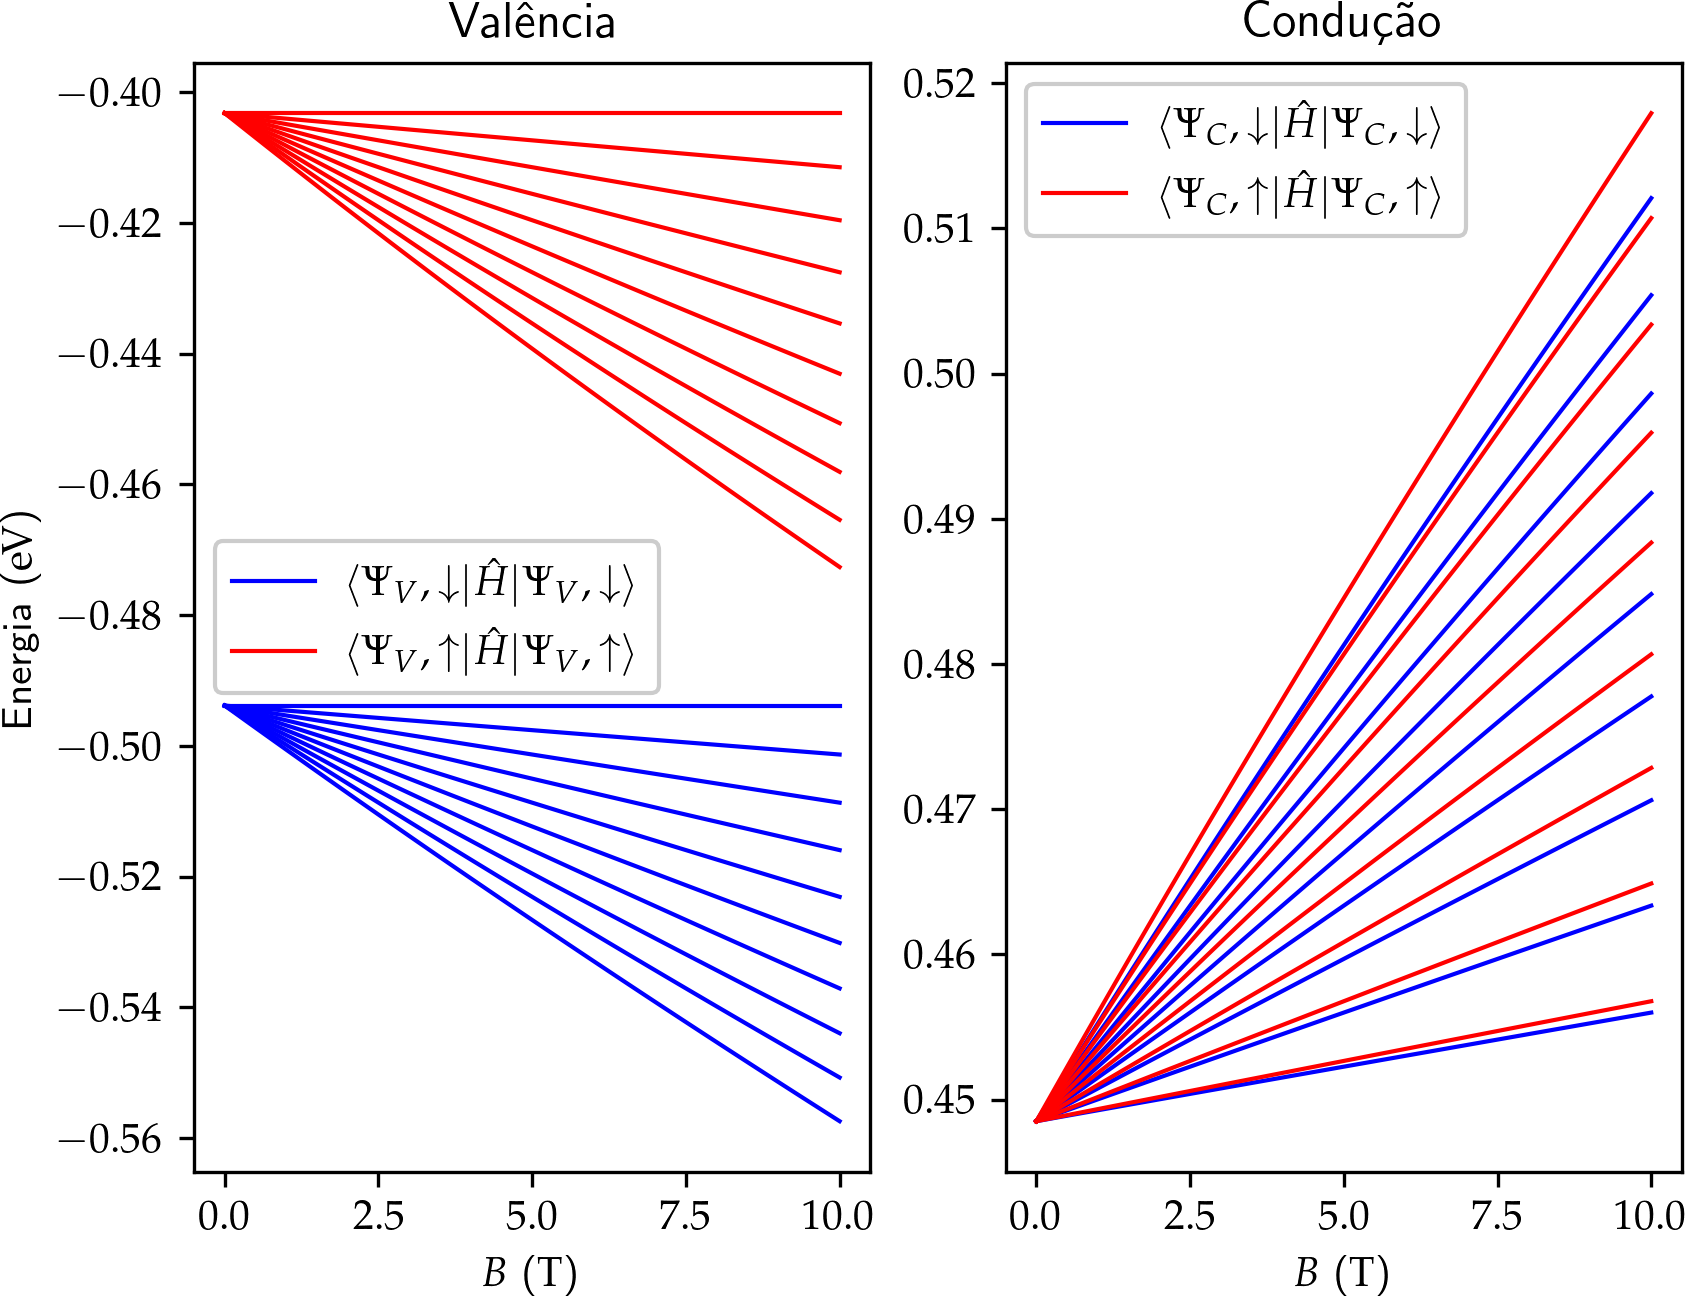
\includegraphics[width=0.68\textwidth]{imagens/crse2_k_valley_landau_levels.png}
    \caption{Níveis de Landau no vale $K$ para \ch{CrSe2} em termos de $B$.}
  \end{figure}
\end{frame}

\begin{frame}{Níveis de Landau}
  \begin{figure}
    \centering
    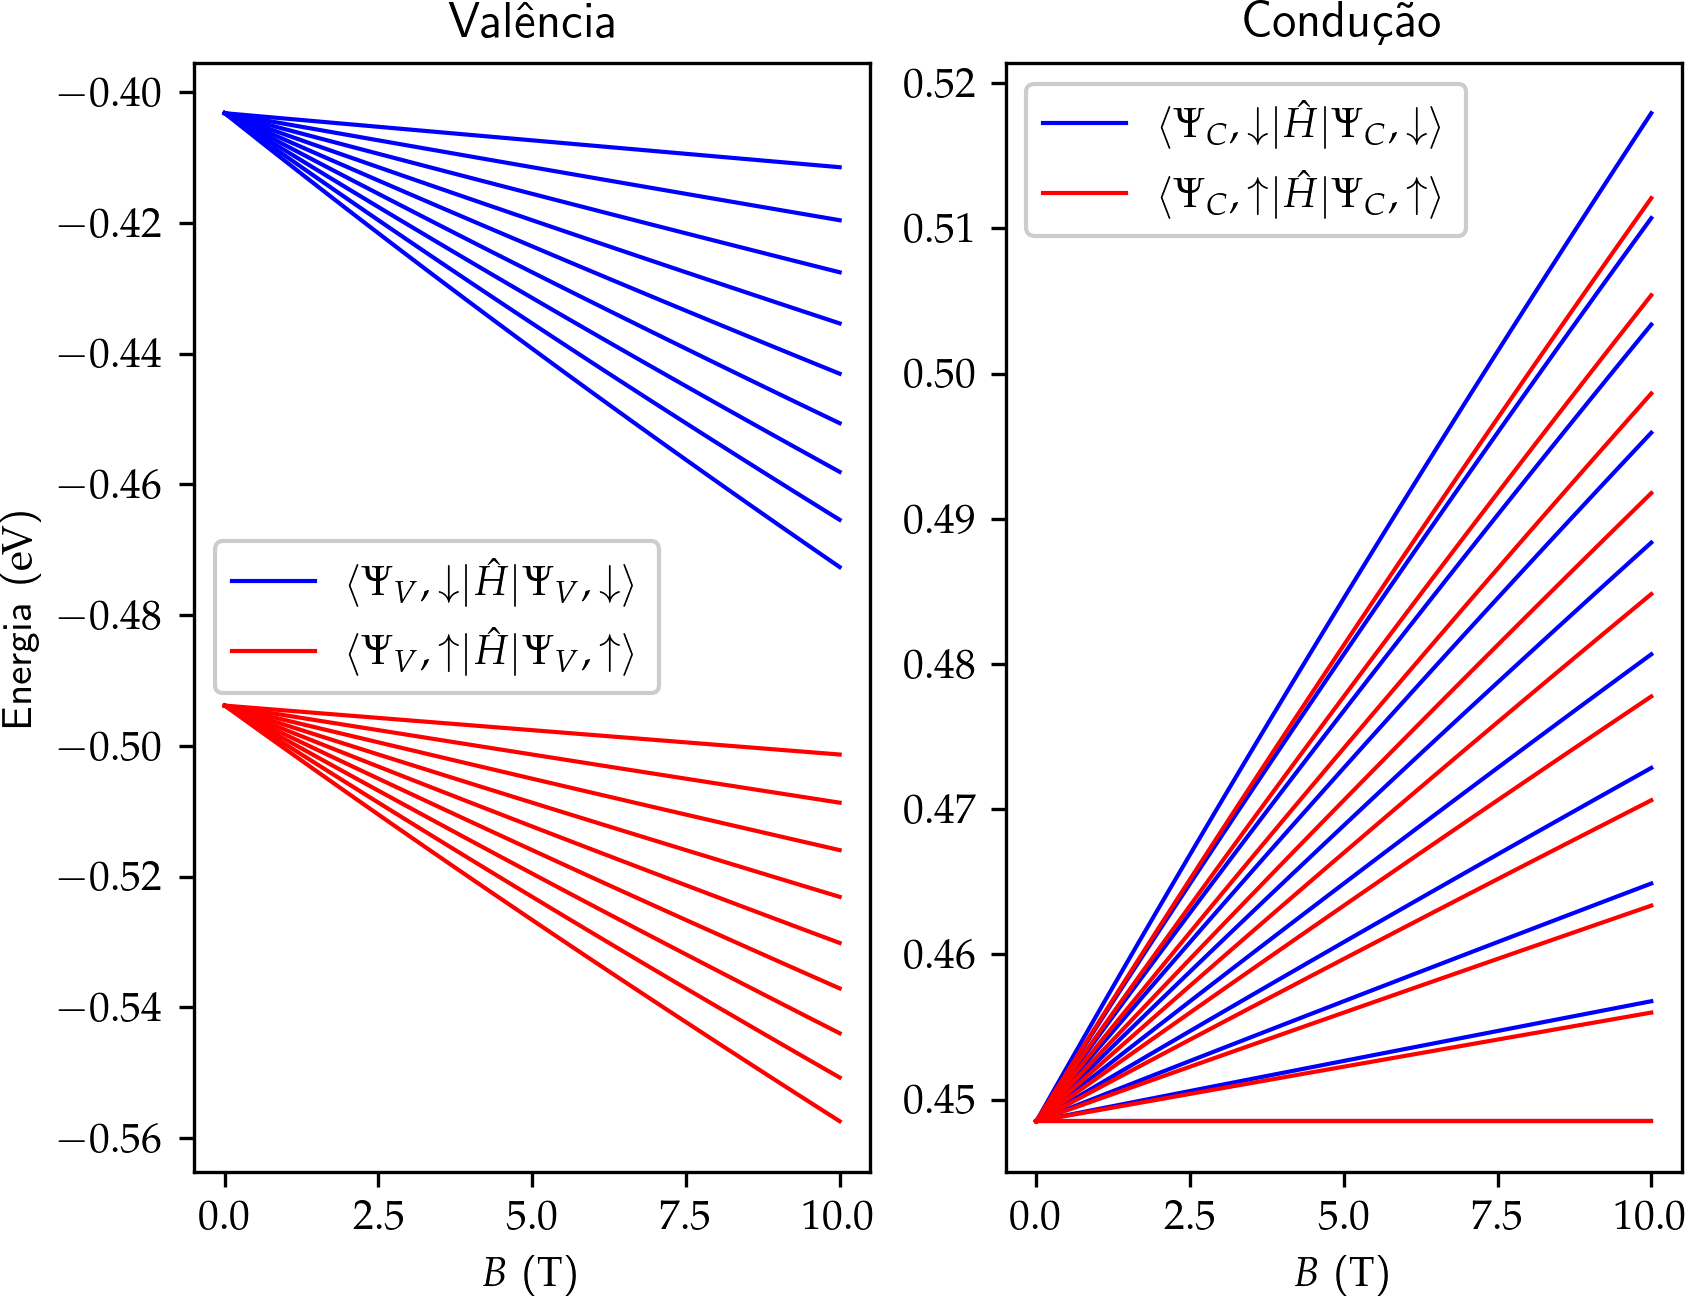
\includegraphics[width=0.68\textwidth]{imagens/crse2_k_prime_valley_landau_levels.png}
    \caption{Níveis de Landau no vale $K'$ para \ch{CrSe2} em termos de $B$.}
  \end{figure}
\end{frame}

\begin{frame}{Níveis de Landau}
  \begin{figure}
    \centering
    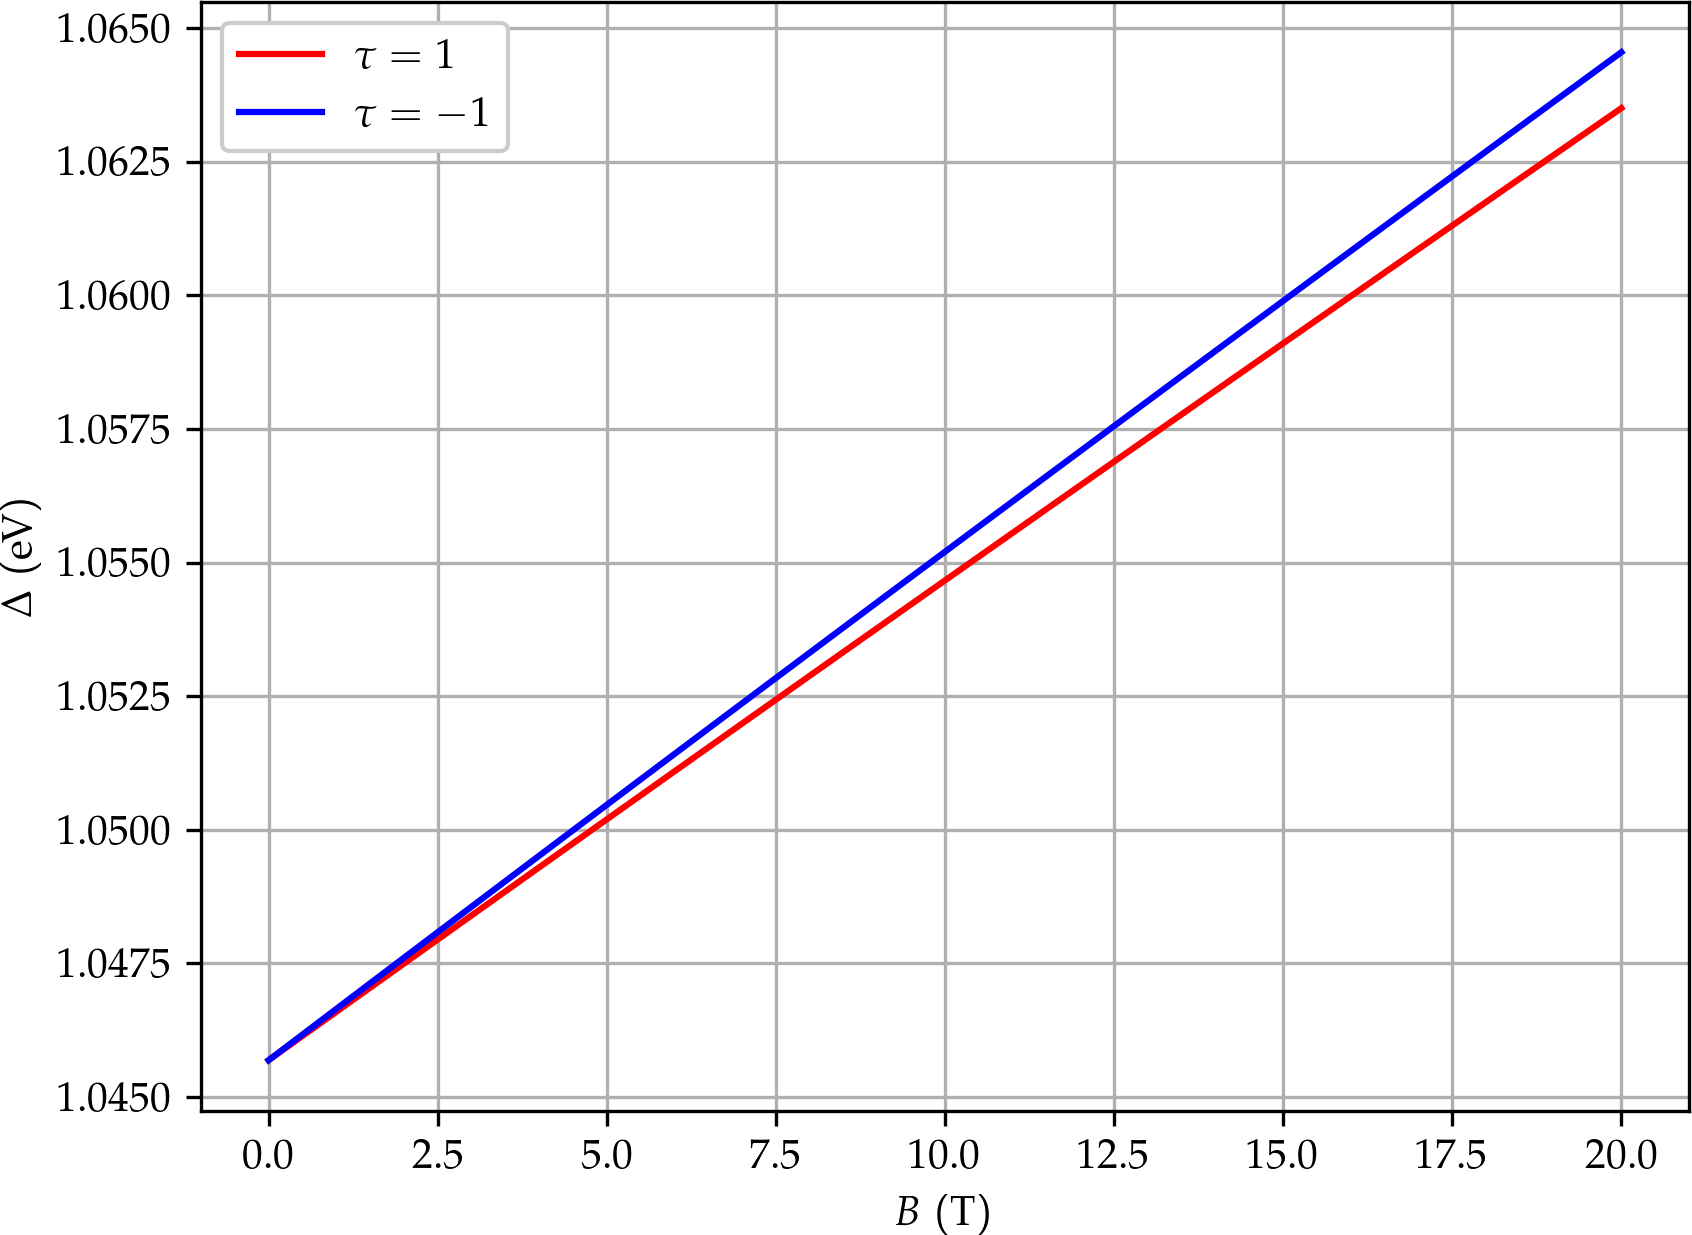
\includegraphics[width=0.68\textwidth]{imagens/crs2_bandgap_field.png}
    \caption{
      Gráficos de $\Delta$ nos vales $K$ e $K'$ para \ch{CrS2} em termos da
      magnitude de $B$.
    }
  \end{figure}
\end{frame}

\begin{frame}{Níveis de Landau}
  \begin{figure}
    \centering
    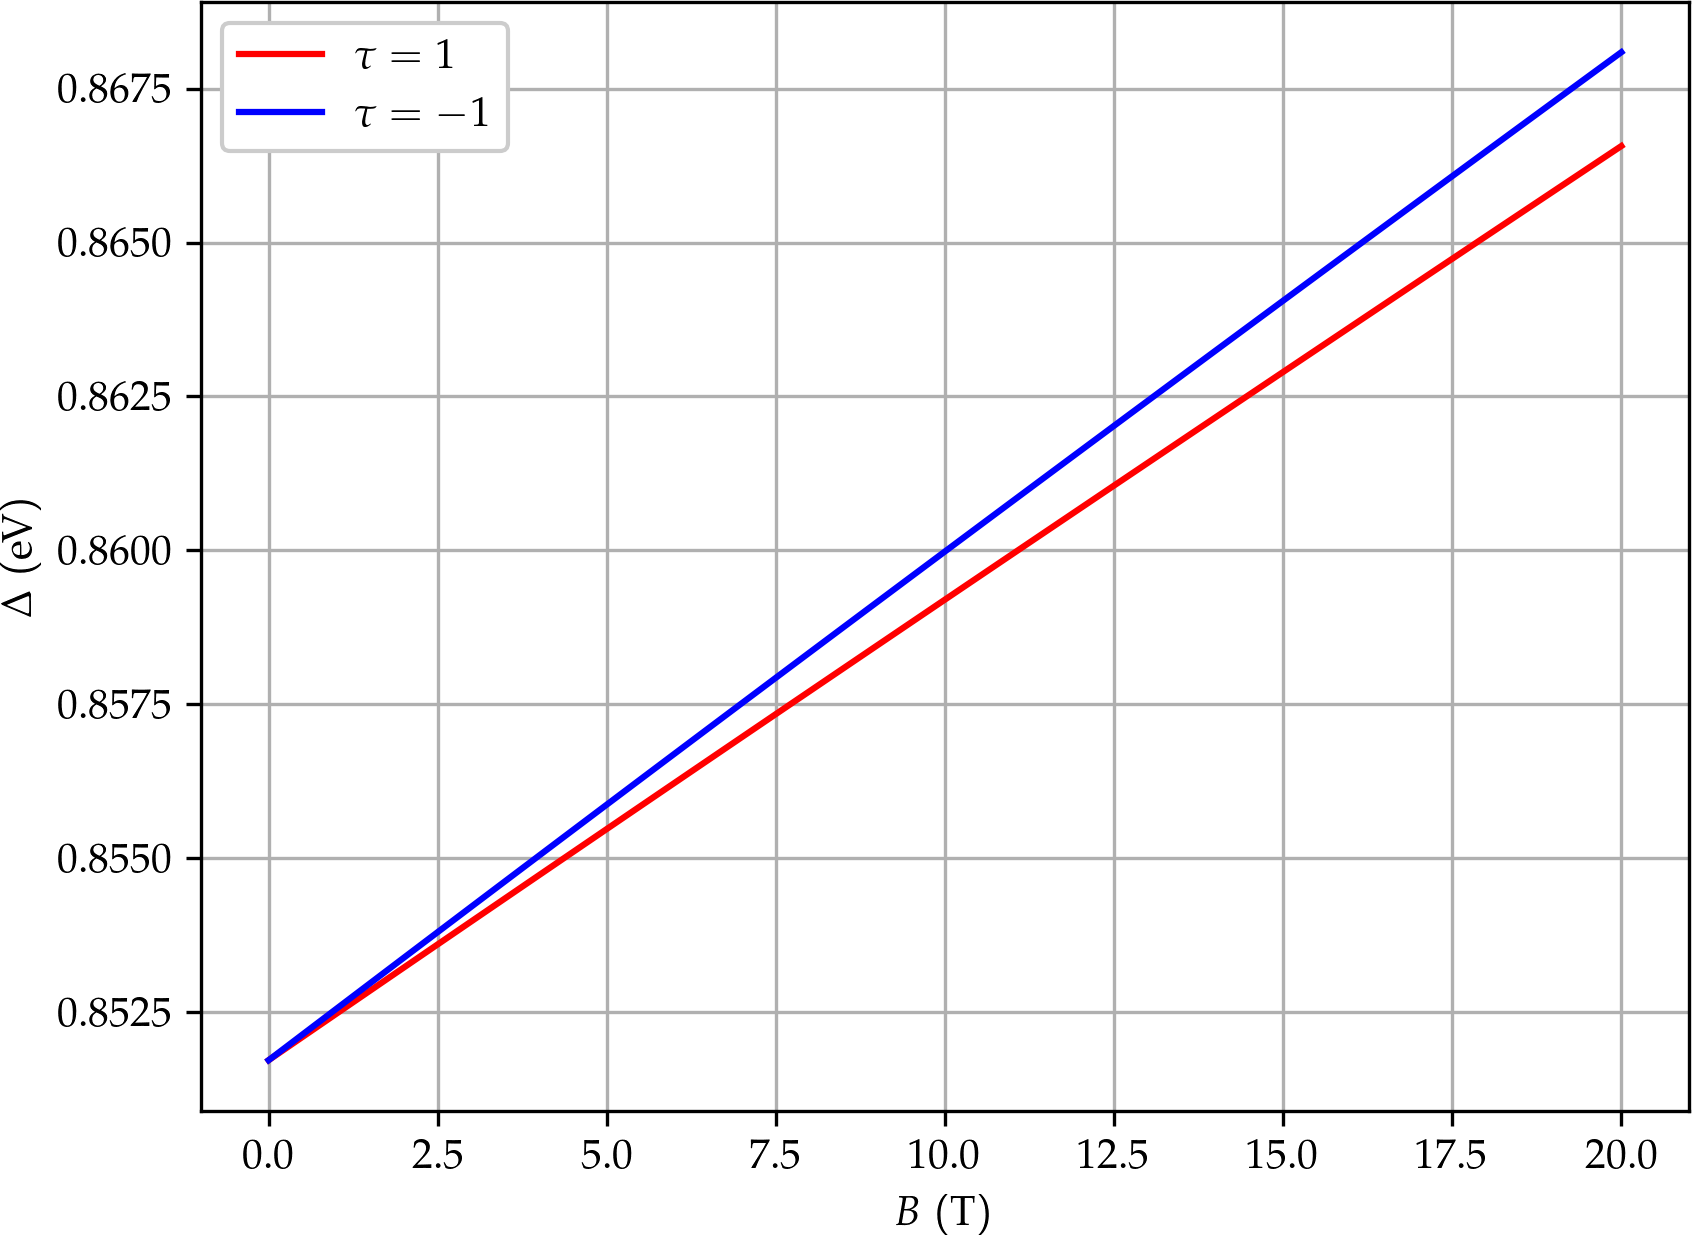
\includegraphics[width=0.68\textwidth]{imagens/crse2_bandgap_field.png}
    \caption{
      Gráficos de $\Delta$ nos vales $K$ e $K'$ para \ch{CrSe2} em termos da
      magnitude de $B$.
    }
  \end{figure}
\end{frame}

\section{Conclusões}

\begin{frame}{Conclusões}
  \begin{itemize}
    \item O algoritmo desenvolvido se mostrou eficaz em espaços de busca de
          dimensões maiores ($\R^{11}$, no problema discutido)
    \item Obteve resultados similares em comparação ao método \textit{Dual Annealing}
    \item O modelo $k \cdot p$ aproximou bem as bandas dos cristais \ch{CrS2} e
          \ch{CrSe2} na vizinhança do vale $K$
    \item Dos parâmetros de ajuste foi possível calcular os níveis de Landau em
          função de $B$ e obter $\Delta (B)$
  \end{itemize}
\end{frame}

\begin{frame}{Conclusões}
  \begin{itemize}
    \item Com a aplicação do campo, há o \textit{splitting} das bandas de
          condução e de valência
    \item Por conseguinte, ocorre uma quebra na simetria de $\Delta$ que antes
          existia entre os vales $K$ e $K'$
    \item Isso abre marge para aplicações que exploram a diferença na
          polarização dos fótons emitidos com a transição de um
          estado de condução para um estado de valência
    \item A polarização do fóton emitido pode ser selecionada com base na
          frequência da luz que incide sobre a monocamada em questão, dada a
          dependência de $\Delta$ com $B$
  \end{itemize}
\end{frame}

\begin{frame}{Conclusões}
  \begin{itemize}
    \item Há uma diferença considerável entre o tempo de execução para o
          Algoritmo Genético e para o \textit{Dual Annealing}
    \item Isso sugere uma implementação em linguagens mais rápidas e que
          permitam uma melhor paralelização do algoritmo, como C, Fortran, Julia ou Go
  \end{itemize}
  \begin{table}
    \centering
    \begin{tabular}{lcc}
      \toprule
                              & 1ª Ordem   & 3ª Ordem   \\
      \midrule
      Algoritmo Genético      & 15 minutos & 25 minutos \\
      \textit{Dual Annealing} & 2 minutos  & 10 minutos \\
      \bottomrule
    \end{tabular}
    \caption{
      Tempo médio de execução do processo de otimização para o Algoritmo
      Genético e para o \textit{Dual Annealing}
    }
  \end{table}
\end{frame}

\section{Referências}

\nocite{dias2016article}
\nocite{dias2016tmdc}
\nocite{kolobov2016tmdc}
\bibliographystyle{abbrv}
\bibliography{bibliografia.bib}
\end{document}